\documentclass[12pt]{article}
\usepackage[margin=1in]{geometry}

%%% Packages %%%
\usepackage{amsmath}
\usepackage{amssymb}
\usepackage{amsthm}
\usepackage{bm}
\usepackage{bbm}
\usepackage{mathtools}
\allowdisplaybreaks

\usepackage{graphicx}
\usepackage{tikz}
\usepackage{float}
\usepackage{enumitem}
\usepackage{booktabs}
\usepackage{pdflscape}
\usepackage{setspace}
\onehalfspacing

% preambles for math writing
\newtheorem{assumption}{Assumption}
\newtheorem{lemma}{Lemma}
\newtheorem{theorem}{Theorem}
\newtheorem{corollary}{Corollary}
\newtheorem{proposition}{Proposition}
\theoremstyle{definition} % Upright text
\newtheorem{definition}{Definition}
\newtheorem{remark}{Remark}

\DeclareMathOperator*{\plim}{plim}
\DeclareMathOperator*{\var}{Var}
\DeclareMathOperator*{\cov}{Cov}
\DeclareMathOperator*{\corr}{corr}
\DeclareMathOperator*{\rank}{rank}
\DeclareMathOperator*{\tr}{tr}

\newcommand{\indep}{\perp \!\!\! \perp}
\newcommand{\R}{\mathbb{R}}
\newcommand{\I}{\mathbbm{1}}
\newcommand{\argmax}{\mathop{\rm arg~max}\limits}
\newcommand{\argmin}{\mathop{\rm arg~min}\limits}

% spacing around equations
\newlength{\myeqskip}
\setlength{\myeqskip}{9pt}
\AtBeginDocument{
	\setlength\abovedisplayskip{\myeqskip}
	\setlength\belowdisplayskip{\myeqskip}
	\setlength\abovedisplayshortskip{\myeqskip-\baselineskip}
	\setlength\belowdisplayshortskip{\myeqskip}
}

% preambles for figures and tables
\usepackage{tocloft}
\usepackage{caption}
\usepackage[labelformat=simple]{subcaption}
\renewcommand\thesubfigure{(\alph{subfigure})}
\usepackage{longtable}
\usepackage{rotating}
\usepackage{threeparttable}
\usepackage{adjustbox}
\DeclareTextFontCommand{\fignotefont}{\normalfont\footnotesize}
\newcommand{\fignote}[2][\linewidth]{
    \begin{minipage}[]{#1}
        \vspace{12pt}
        \fignotefont{#2}
    \end{minipage}}
\DeclareTextFontCommand{\tabnotefont}{\normalfont\footnotesize}
\newcommand{\tabnote}[2][\linewidth]{
    \begin{minipage}[]{#1}
        \vspace{12pt}
        \tabnotefont{#2}
    \end{minipage}}
\renewcommand\theContinuedFloat{\Alph{ContinuedFloat}}

% path for input files (tables and single num tex files)
\makeatletter
\def\input@path{{../output/}}
\makeatother

% path for figures
\graphicspath{{../output/figure/}}

% preambles for references
\usepackage{natbib}
\usepackage{hyperref}
\hypersetup{colorlinks,citecolor=blue,filecolor=red}
\usepackage{cleveref}

% preambles for cross-referencing
\usepackage{xr-hyper}
\externaldocument[appx-][nocite]{Hara_RenewableRiskSharingAuction_OnlineAppendix}

\title{Encouraging Renewable Investment:\\Risk Sharing Using Auctions\thanks{
I am especially grateful to Ashley Langer, Hidehiko Ichimura, Ryan Kellogg, Derek Lemoine, Juan Pantano, and Matthijs Wildenbeest for their feedback, support, and guidance. I would also like to thank Natalia Fabra, Keisuke Ito, Koichiro Ito, Yuki Ito, Kei Kawai, Eric Richert, Eduardo Souza-Rodrigues, and Mo Xiao for helpful discussions, and the seminar participants at UArizona, UChicago, Michigan State, Osaka University, Western Michigan, Arizona ENREE, IIOC, MSU/UM EEE for many useful comments and suggestions.
This work was supported in part through computational resources and services provided by the Institute for Cyber-Enabled Research at Michigan State University.
All errors are my own.
}}
\author{Konan Hara\footnote{Department of Economics, Michigan State University. Email: harakon1@msu.edu}}

\date{\today}

\begin{document}

\maketitle

\begin{abstract}
\onehalfspacing
Renewable energy investors commit to high upfront capital costs while facing highly uncertain returns from wholesale electricity sales. I estimate the joint distribution of investors' risk aversion and costs from the investors' portfolio choices in Brazil's wind power purchase agreement auctions. To entice investors to install wind turbines costing \$\input{snt/total_cost_sb_nomissing} billion, the policymaker would spend \$\input{snt/total_rp_sb_nomissing} billion less in expectation by taking on all wholesale market risk rather than leaving it with investors. Counterfactuals examine the consequences of implementing risk sharing using alternative auction designs when the policymaker does not know investors' risk aversion and costs ex-ante.
\end{abstract}

\noindent \textbf{Keywords}: Renewable energy investment, wholesale electricity markets, purchase agreement, risk-averse bidders, multidimensional bids

% \noindent \textbf{JEL Codes}: TBW

\clearpage

\section{Introduction}

Widespread private sector investment in renewable energy is crucial in mitigating the impacts of climate change \citep{REN212023}. Renewable energy investors expect financial returns from sales of electricity produced from new renewable capacity. However, wholesale electricity markets have volatile prices, and investors cannot shift their production schedule to avoid low prices because of the intermittency of renewable energy \citep{Beiter2024}. Moreover, renewable technologies are much more capital-intensive than fossil fuel-based plants, where fuel costs dominate the overall costs \citep{Schmidt2014}. High upfront capital costs of new renewable capacity can make investors substantially risk-averse to uncertain revenues \citep{May2021}. The situation would worsen in low and middle-income countries with under-developed financial markets where handing off the risk to financial entities is costly \citep{Ameli2021,Calcaterra2024}. Therefore, policymakers' risk-sharing can be essential in promoting renewable investments unless private markets can absorb the risk at a modest cost \citep{Schmidt2014,Beiter2024}.

% worldwide renewable energy targets
% 174 countries have set renewable energy targets, and 128 have set economy-wide targets.

% worldwide volatile wholesale electricity prices
% \footnote{
% Volatile wholesale electricity prices are prevalent worldwide: for recent examples, see European Commission (2022) and EIA (2023) for the volatile prices in 2022 in the EU and U.S., respectively.
% % cite: https://commission.europa.eu/news/high-volatility-and-geopolitical-tensions-impact-electricity-and-gas-market-developments-q1-2022-2022-07-08_en
% % cite: https://www.eia.gov/todayinenergy/detail.php?id=55139
% }

Policymakers have implemented two broad approaches to aid renewable investors financially: power purchase agreements and generation subsidies \citep{IRENA2019}.\footnote{
Purchase agreements and subsidies are also called feed-in tariffs and feed-in premiums. Also, my framework can handle upfront investment subsidies instead of generation subsidies. The policy implications are the same if the upfront subsidy equals the present value of the generation-subsidy payments and neither payment arrangement entails payout risk.
} Purchase agreements ensure a certain price regardless of wholesale prices, while subsidies pay a premium on top of wholesale prices, creating a critical difference in who bears the wholesale market risk (\citealp{Farrell2017}; \citealp*{Alcorta2023}). With purchase agreements, policymakers take the risk from investors, while the risk remains on the investors' side with subsidies. Consequently, policymakers face a trade-off between taking the risk and paying investors to assume the risk, corresponding to investors' \textit{risk premiums}. I estimate investors' risk premiums from their \textit{portfolio choices}, providing the policymaker with a menu of possible cost-risk combinations for supporting renewable investment. I then examine the consequences of implementing risk sharing using auctions when the policymaker does not know investors' risk premiums and costs \textit{ex-ante}. Recent work highlights that private long-term purchase agreements can be constrained by counterparty and renegotiation risk, motivating a larger role for regulator-backed arrangements \citep{Fabra2025a,Fabra2025b}.

I study the trade-off using long-term wind power purchase agreement auctions, planned and administered by the Brazil Ministry of Mines and Energy (Minist\'erio de Minas e Energia, MME) and Electricity Regulatory Agency (Ag\^encia Nacional de Energia El\'etrica, ANEEL), respectively, from \input{snt/auction_year_min} to \input{snt/auction_year_max}. MME calls for investors with a new wind turbine installation project to bid 1) a share of the production they will include in a purchase agreement and 2) a price for each unit of this share. The lowest bid prices win the purchase agreements until the auction's procurement capacity is reached, with ANEEL guaranteeing payouts for 20 years---the wind turbines' lifetime. In exchange, winners commit to installing their planned capacity. Winners secure a purchase agreement for the share of the production they bid and sell the remaining production into Brazil's wholesale market, consisting of a spot market, short-term purchase agreements intermediated by ANEEL, and bilateral contracts with high-volume consumers \citep{Hochberg2021}. The short-term purchase agreements and bilateral contracts usually last up to 6 years \citep{CCEE2024,Perez2024}, leaving prices uncertain upon renewal. Moreover, ANEEL has been concerned about the transparency of price formation and counterparty risks in payouts in bilateral contracts \citep{CCEE2012}. The uncertain prices and counterparty risks motivated MME to provide long-term purchase agreements immune from these wholesale market risks to ease investors' upfront capital financing \citep{Tolmasquim2021}.

Bidders essentially make portfolio choices to allocate their total production across the risk-free purchase agreement and risky wholesale market. I use these portfolio choices to recover the overall premium for wholesale market risk, bundling price volatility, contract-renewal uncertainty, and counterparty risk---whereas \citet{Ryan2026} quantifies the premium for state-government counterparty risk by comparing Indian solar auctions intermediated by state and central governments.\footnote{
Researchers have used structural models to value risks affecting energy investment, exploiting intertemporal or cross-sectional variation in uncertainty to identify investors' responses to different levels of risk (e.g., \citealp{Kellogg2014}; \citealp{Chen2024}; \citealp*{Gowrisankaran2025}; \citealp{Ryan2026}). I instead use portfolio choices to recover the overall premium investors require for residual exposure outside a long-term contract.
} This approach is useful when investors face multiple interacting risks and policymakers care about de-risking the overall revenue stream \citep{Fabra2025a}.

Portfolio choices embedded in auctions can indicate bidders' risk attitudes, as \citet{Athey2001} have noted in scaling auctions. Risk-neutral bidders will allocate all of their allocatable production to either the purchase agreement or wholesale market, whichever gives them the higher expected price. However, \input{snt/bidder_prop_partial} of bidders in the data make partial allocations. These partial allocations are consistent with risk-averse bidders diversifying their portfolios to balance expected price and price variability. Motivated by this observation, I develop a structural model of risk-averse bidders in these auctions to separately recover bidders' expected wholesale price, risk premiums, and private costs, following the share auction framework of \citet{Wilson1979}. I extend \citet{Bolotnyy2023} and \citet{Luo2024}'s identification strategies in scaling auctions to a different auction design involving bidders' portfolio choices more explicitly.\footnote{
See \citet{Perrigne2019} and \citet{Vasserman2021} for literature reviews on identifying bidders' risk aversion.
}

Bidders with heterogeneous risk aversion and cost types, sharing a common expected wholesale price belief, choose their bid share and price to maximize expected utility. Conditional on the bidder's bid price, the bid share does not affect the likelihood of winning, so the share decision is a portfolio choice between a risk-free purchase agreement and a risky wholesale market conditional on winning. Given the wholesale price variability quantified from market data, bidders' trade-offs between expected price gains and additional price variability across purchase agreement prices identify their risk aversion. The minimum purchase agreement price at which bidders allocate all production to the purchase agreement also informs the expected wholesale price because bidders prefer a risk-free price to a risky alternative with the same expected price. My framework does not require computing investors' expected wholesale prices directly from detailed wholesale market data---which are difficult to collect because many transactions involve private bilateral contracts. Even when such data are available, a finite historical sample may provide limited guidance about investors' price expectations over a 20-year horizon.

I employ statistical properties of the \textit{concomitants} of order statistics \citep{Yang1977} to show that winners' bids and attributes identify their participant distribution when winners are selected on a one-dimensional ranking variable. Having access only to winners' bids is common in new renewable energy auctions because policymakers are concerned about the future competition impacts of making all bids public.\footnote{
MME raises this concern as the primary reason for not making their auction participant generation cost microdata public \citep{EPE2022b}.
}
Under the i.i.d. draws implied by symmetric bidders, the conditional distribution of the remaining bid components and bidder attributes given bid price is the same among winners and participants. Intuitively, ranking bidders by price preserves the pairing between each price and the bidder's other bid components and attributes, so conditioning on price leaves their relationship unchanged. This extends the recovery of one-dimensional bid distributions from winners \citep{Athey2002} to multidimensional bids and bidder attributes.

I establish identification for the sealed-bid and descending-clock auction formats observed in the data. Sealed-bid participants submit a one-shot bid whose share and price jointly reflect their risk aversion and cost. A descending-clock auction instead reveals the marginal loser's bid price as the clearing price, while winners choose their shares before this price is known. Estimation proceeds in two steps. I first estimate the risk aversion distribution and expected wholesale price from the bid share optimality condition using the generalized method of moments. I then recover costs by combining the inferred participant distribution with the optimal bid price condition in the spirit of \citet*{Guerre2000}. I use both auction formats in the first step but only sealed-bid auctions in the second because a descending-clock auction reveals only one clearing price, which informs the cost of the marginal bidder rather than the individual costs of all winners.

I find that the average winner's risk premium from selling all electricity into the wholesale market is \$\input{snt/rp_mean_winner}/MWh, or \input{snt/rp_cost_ratio_mean_winner} of the estimated cost of \$\input{snt/cost_mean_winner}/MWh. This revealed-preference estimate is comparable to \citet{May2021}'s estimate, based on interviews and a model of financing costs, that financing costs increase European renewable energy deployment costs by 29\%. For the \input{snt/total_capacity_sb_nomissing} GW of winning projects included in the cost estimation, the aggregate risk premium is \$\input{snt/total_rp_sb_nomissing} billion relative to an aggregate estimated cost of \$\input{snt/total_cost_sb_nomissing} billion. Taking on all wholesale market risk through full share purchase agreements would reduce the policymaker's expected expenditure by this \$\input{snt/total_rp_sb_nomissing} billion relative to a subsidy, but the associated discounted wholesale revenue has an expected value of \$\input{snt/total_wholesale_revenue_mean_sb_nomissing} billion and a standard deviation of \$\input{snt/total_wholesale_revenue_sd_sb_nomissing} billion over 20 years. The policymaker's distaste for this revenue risk can depend on how she recoups losses from risk-taking, often through a surcharge on consumers' bills, as in Brazil \citep{Tolmasquim2021},\footnote{
A renewable energy surcharge is a common way to fund financial aid on renewable investments worldwide, including in Canada, China, Germany, Ireland, Italy, Japan, and the United Kingdom \citep{Ming2013,Ansarin2022}.
} or direct tax \citep{Beiter2024}.

Given investors' risk premiums and costs, the policymaker can choose how much wholesale market risk to take on according to her own attitude toward risk. Auctions provide a practical way to implement risk sharing when she does not know investors' premiums and costs accurately \textit{ex-ante}. Indeed, future wind technology cost declines are uncertain and difficult to forecast accurately \citep{Wiser2021}. Moreover, as costs decline, wind power investment without policymaker support becomes viable, reducing the incremental value of support through such auctions. I compare two auction designs for implementing risk sharing in this environment. Brazilian new energy auctions allow bidders to individually choose their purchase agreement shares, which effectively lets them choose how much wholesale market risk to retain---I refer to this design as \textit{bidder share choice}. Alternatively, in \textit{fixed share auctions}, the policymaker chooses the proportion of wholesale market risk she takes on by imposing the same purchase agreement share on all bidders. These auctions encompass subsidies and full share purchase agreements as two extremes, with the policymaker taking none or all of the wholesale market risk, respectively. I extend the model to allow endogenous auction participation and calibrate the qualification cost to match the observed participation rate among registered projects, following \citet{Bolotnyy2023}.

The counterfactuals show that average winner risk aversion rises once construction without auction support becomes viable, because low risk aversion bidders find this outside opportunity more attractive and value winning less. By contrast, a smaller purchase agreement share in fixed share auctions shifts awards toward low risk aversion investors because greater wholesale market exposure makes more risk-averse bidders less willing to bid aggressively, potentially disadvantaging smaller or less diversified developers if they are more risk averse \citep*{Herranz2015}. Bidder share choice moderates this distributional effect by allowing support to decline according to each bidder's need for revenue stabilization. However, decentralizing portfolio choice through bidder share choice comes at a cost because winners retain part of the value of portfolio flexibility as a markup. Holding the policymaker's wholesale market risk exposure constant, a fixed share auction generally lowers the winner markup and the resulting policy cost---the aggregate markup difference amounts to \$\input{snt/cf_matched_markup_gap_m6_million} million for wind turbines costing \$\input{snt/cf_choice_winner_cost_m6_billion} billion.

The methodology developed in this paper can be used to quantify investors' risk premiums and evaluate risk sharing in electricity markets beyond Brazil. Policymakers can elicit the required portfolio choices by asking investors to bid shares as well as prices in long-term purchase agreement auctions used across renewable technologies worldwide \citep{IRENA2019,IRENA2024a}. The European Commission's hydrogen auctions already allow investors to choose their shares \citep{EuropeanCommission2024}. The framework also applies to other investments with positive externalities and high risk premiums associated with uncertain returns, such as carbon markets and transmission lines \citep{FederalGovernmentofGermany2023,DOE2023}.

% [Other recent examples]
% carbon contracts for difference in Germany
% capacity contracts in the U.S. Department of Energy Transmission Facilitation Program

% [Subsidies and purchase agreements]
% 83 countries have adopted generation subsidies or purchase agreements (REN21, 2023).
% Historically, the U.S. prefers subsidies, while purchase agreements are much more popular in other countries supporting renewable investment (Schmalensee, 2012). (This might be because the investors' risk premiums is low in the U.S.)

% [reasons why private financial markets may not exist]
% There are several reasons why private financial markets may not function as a risk-sharing tool in the context of renewable investments. First, the long-term nature of renewable investments may make the existence of private financial markets difficult. Second, risk pooling may unravel due to the high correlation of the wholesale market risk across projects. Third, annual spot prices are positively correlated with GDP (correlation coefficient 0.38 from 2001--2022), which makes hedging more difficult.

The remainder of the paper proceeds as follows. Section \ref{sec:theory} presents a simple model of risk sharing between a policymaker and a renewable investor. Section \ref{sec:contextdata} describes Brazil's new energy auctions and the data. Sections \ref{sec:model} and \ref{sec:econometric} present the structural model, identification, and estimation. Section \ref{sec:results} reports the structural estimates, Section \ref{sec:counterfactuals} presents the counterfactual analysis, and Section \ref{sec:conclusion} concludes.

\section{Theoretical Framework of Risk Sharing}
\label{sec:theory}

I present a simple model of risk sharing between a policymaker and a renewable investor. The investor has a potential project that costs $c$, generates a certain amount of electricity, and yields risky lifetime wholesale market revenue $r$ without policy support. The investor has increasing and weakly concave utility $u$ over project profit $\pi$, normalized so that $u(0)=0$. A risk premium for profits $\pi$, $RP_\pi \geq 0$, satisfies $E[u(\pi)] = u(E[\pi] - RP_\pi)$, so the certainty equivalent is $\mathrm{CE}(\pi)\coloneqq E[\pi]-RP_\pi$. I additionally assume that certainty equivalents are invariant to additive shifts by a certain payoff, $\mathrm{CE}(\pi+a)=\mathrm{CE}(\pi)+a$ for any certain $a$. Thus, for a given investor and wholesale market exposure, a certain contract payment shifts the certainty equivalent one-for-one without changing the associated risk premium. This property holds under the constant absolute risk aversion (CARA) preferences used in the structural model in Section \ref{sec:model} and does not restrict the cross-sectional relationship between investors' risk premiums and project costs. A risk-neutral investor's risk premium is zero for any distribution of $\pi $. A strictly risk-averse investor's risk premium increases under a mean-preserving spread and is zero if and only if $\pi $ is certain. In this benchmark, investment is not viable without policymaker support, so the investor does not build and earns a certainty equivalent of zero.\footnote{The structural model in Section \ref{sec:model} relaxes this assumption by allowing a nonzero outside payoff.}

The policymaker values the renewable project sufficiently to induce its construction. Knowing that the investor can be risk-averse, the policymaker considers a contract that shares the market risk between her and the investor to support the investment. This risk-sharing contract consists of three elements. First, the policymaker pays a certain amount $\phi$ to the investor. Second, the investor commits to building the planned renewable project. Third, the investor provides the policymaker with a share $\lambda \in [0,1] $ of the lifetime electricity. This contract encompasses the two commonly adopted renewable support schemes, a full share purchase agreement at $\lambda = 1 $ and a subsidy at $\lambda = 0 $, as the two extremes.\footnote{
Another common scheme, a contract for differences, guarantees a minimum price and falls between these extremes because the policymaker takes on part of the investor's wholesale market risk.
} Under the contract, the investor is only responsible for selling a share of $1 - \lambda $ of the electricity to the wholesale market. The investor signs the contract when it gives a non-negative expected utility:
\begin{align}
\label{eq:contract}
E[u(\phi + (1-\lambda) r - c)] \geq 0 \iff \underbrace{\phi + (1-\lambda) E[r]}_{\text{Expected revenue}} \geq \underbrace{c}_{\text{Cost}} + \underbrace{RP_r(1-\lambda)}_{\substack{\text{Wholesale market} \\ \text{risk premium}}},
\end{align}
where $RP_r(1-\lambda) \coloneqq RP_{(1-\lambda)r} $ is the investor's risk premium for selling share $1 - \lambda $ of the electricity to the wholesale market. When the investor sells no electricity to the wholesale market, the revenue is certain and his risk premium is zero, \(RP_r(0)=0\). I assume that the risk premium increases with the share sold to the wholesale market, \(RP_r'(1-\lambda)>0\), as it does under the CARA specification used in the structural model.

Having decided to induce construction, the policymaker minimizes the required support by setting the contract payment \(\phi\) to the lowest amount the investor is willing to accept. Thus, the contract acceptance condition in equation~\eqref{eq:contract} binds, and the investor earns a certainty equivalent of zero. The policymaker sells a share \(\lambda\) of the electricity to the wholesale market, yielding revenue of \(\lambda r\). Since the policymaker pays the contract payment \(\phi(\lambda)\), her net expenditure is \(NE(\lambda)=\phi(\lambda)-\lambda r\). The policymaker evaluates the risk associated with the contract by the variance of the net expenditure. Substituting the value of $\phi$ and taking expectation and variance, I obtain the policymaker's cost-risk trade-off:
\begin{align}
\label{eq:tradeoff}
E[NE(\lambda)] = \underbrace{c - E[r]}_{\text{Cost compensation}} + \underbrace{RP_r(1-\lambda)}_{\text{Investor's risk premium}}
\text{ and }
\var(NE(\lambda)) = \underbrace{\lambda^2 \var(r)}_{\text{Policymaker's risk}}.
\end{align}
Expected net expenditure equals project cost net of expected wholesale revenue plus compensation for the investor's remaining wholesale market risk. It falls as $\lambda $ rises, while the variance borne by the policymaker increases as $\lambda^2\var(r) $. Thus, the subsidy at $\lambda=0 $ has the highest expected net expenditure and zero variance, whereas the full share purchase agreement at $\lambda=1 $ minimizes expected net expenditure and transfers all wholesale market risk to the policymaker (Figure \ref{fig:tradeoff}). The difference in expected net expenditure between these policies equals the investor's risk premium for selling all electricity to the wholesale market, $RP_r(1) $. If the investor is risk-neutral, $RP_r(1-\lambda)=0 $ for any $\lambda $, so expected net expenditure does not vary with risk sharing and the policymaker faces no cost-risk trade-off.

\begin{figure}[htb!]
\caption{Policymaker's cost-risk trade-off from risk-sharing contracts}
\label{fig:tradeoff}
\centering
\resizebox{\textwidth}{!}{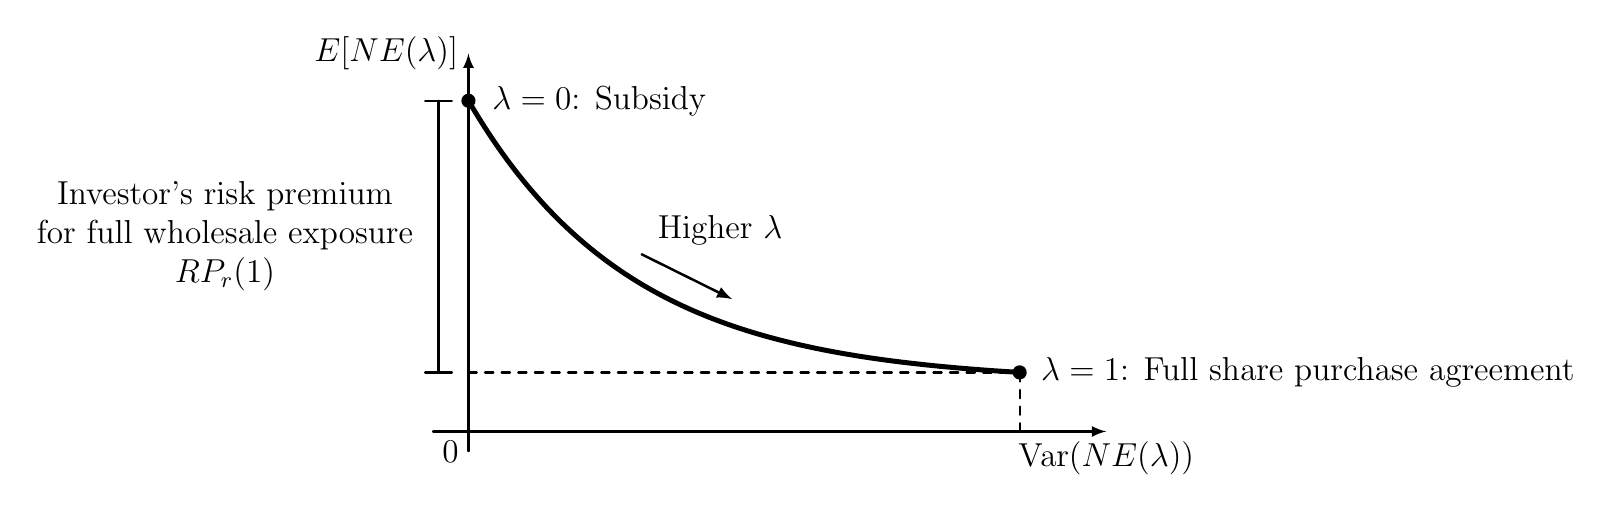
\begin{tikzpicture}[x=1cm,y=1cm,>=latex,line cap=round,line join=round]
  % Axes
  \draw[->, line width=0.8pt] (-0.45,0) -- (8.1,0)
    node[below,font=\large] {$\var(NE(\lambda))$};
  \draw[->, line width=0.8pt] (0,-0.25) -- (0,4.8)
    node[left,font=\large] {$E[NE(\lambda)]$};

  % Reference levels
  \draw[dashed, line width=0.8pt] (0,0.75) -- (7.0,0.75);
  \draw[dashed, line width=0.8pt] (7.0,0) -- (7.0,0.75);

  % Policymaker cost-risk frontier
  \draw[line width=1.8pt]
    plot[domain=0:7.0,samples=100]
    (\x,{0.75 + 3.45*(exp(-0.48*\x)-exp(-0.48*7))/(1-exp(-0.48*7))});

  % Endpoints
  \fill (0,4.20) circle (0.09);
  \fill (7.0,0.75) circle (0.09);

  % Risk-premium between the two endpoints
  \draw[line width=0.8pt] (-0.38,0.75) -- (-0.38,4.20);
  \draw[line width=0.8pt] (-0.55,0.75) -- (-0.21,0.75);
  \draw[line width=0.8pt] (-0.55,4.20) -- (-0.21,4.20);
  \node[align=center,left,font=\large] at (-0.58,2.48)
    {Investor's risk premium\\for full wholesale exposure\\$RP_r(1)$};

  % Labels
  \node[below left,font=\large] at (0,0) {$0$};
  \node[align=left,right,font=\large] at (0.18,4.20)
    {$\lambda=0$: Subsidy};
  \node[align=left,right,font=\large] at (7.15,0.75)
    {$\lambda=1$: Full share purchase agreement};

  \draw[->, line width=0.9pt] (2.2,2.25) -- (3.35,1.68);
  \node[above right,font=\large] at (2.28,2.25) {Higher $\lambda$};
\end{tikzpicture}
}
\fignote{Notes: Moving right increases the variance of the policymaker's net expenditure, $\var(NE(\lambda))$, while moving down lowers expected net expenditure, $E[NE(\lambda)]$, by reducing the investor's required risk premium compensation. The vertical distance between the subsidy and full share purchase agreement endpoints equals the investor's risk premium from bearing all wholesale market risk, $RP_r(1)$.}
\end{figure}

The policymaker chooses $\lambda $ to balance her expected net expenditure and risk according to her preferences and institutional or political constraints. I define the sum of expected net expenditure and the policymaker's risk premium as her certainty equivalent net expenditure. Absent additional constraints, she solves $\min_{\lambda \in [0,1]} \left\{E[NE(\lambda)] + RP_r^{PM}(\lambda)\right\}$, where $RP_r^{PM}(\lambda) \coloneqq RP_{\lambda r}^{PM} $ is the policymaker's risk premium for selling the contracted electricity to the wholesale market.\footnote{
With a certain budget, minimizing certainty equivalent net expenditure is equivalent to maximizing the policymaker's expected utility over the budget remaining after net expenditure.
} The policymaker solves the problem using the expected net expenditure formula in equation~\eqref{eq:tradeoff}. A risk-neutral policymaker ($RP_r^{PM}(\lambda) = 0 $ for any $\lambda $) takes all risks ($\lambda = 1 $) if the investor is risk-averse. For a risk-averse policymaker, I assume that the risk premium functions for the policymaker and investor are increasing, differentiable, and convex. For instance, these conditions hold when risk premiums are proportional to the variance of wholesale market exposure, as under the CARA preferences and normally distributed \(r\) used in the structural model. An interior optimum balances the marginal risk premiums of the policymaker and investor, $(RP_r^{PM})'(\lambda) = RP_r'(1-\lambda) $. If their risk premium functions are identical and the objective is strictly convex, the unique optimum is $\lambda=1/2 $. I assess the welfare consequences of risk-sharing contracts using this certainty equivalent, consistent with the U.S. Office of Management and Budget's recent proposal to use certainty equivalents when accounting for uncertainty in Federal activities \citep{OMB2023}.

% source of policymaker's risk aversion
% The policymaker can be risk-averse because of a ``fiscal risk management'' motive (Hanson, Scharfstein, \& Sunderam, 2019).
% In contrast, the policymaker can be less risk-averse because it can diversify its portfolio more through various public projects and have looser liquidity constraints by intergenerational risk sharing (Arrow \& Lind, 1970; Falkenheim, 2021).

In practice, the policymaker does not observe investors' costs or attitudes toward wholesale market risk. An auction uses competition to allocate purchase agreements among investors requiring less support, although winners may retain markups whose size depends on the auction format and competitiveness. Brazilian auctions are particularly informative because bidders choose both a purchase agreement price and the share of electricity sold under the purchase agreement, choices that jointly reflect investors' costs and risk premiums. Recovering both is necessary to distinguish the resource cost of renewable investment from the compensation investors require for bearing risk and, therefore, to evaluate the policymaker's cost-risk trade-off under alternative risk-sharing policies.

\section{New Energy Auctions in Brazil}
\label{sec:contextdata}

% [renewable energy auctions globally]
% Renewable energy auctions procure electricity from renewable technologies to support their investments. The number of countries that have held renewable energy auctions reached 106 by the end of 2018, and the estimated total capacity of 110.6 GW was auctioned in 2017--2018 globally (IRENA, 2019). The major technologies are solar (52\%) and onshore wind (36\%), and offshore wind is expanding its share (9\%).

Since 2005, MME and ANEEL have organized long-term power purchase agreement auctions to contract new renewable generation capacity across multiple auction types---New Energy Auctions (Leil\~ao de Energia Nova), Alternative Sources Auctions (Leil\~ao de Fontes Alternativas), and Reserve Energy Auctions (Leil\~ao de Energia de Reserva)---covering hydro, biomass, wind, and solar. While Brazil had historically relied on abundant hydropower, expanding non‑hydro renewables became essential for several reasons \citep{Werner2023}. First, it became increasingly difficult to build new large-scale hydroelectric capacity to meet the expanding demand for electricity and sustain economic growth without affecting the Amazon rainforest's ecology. Thus, expanding the renewable capacity beyond hydro was crucial to avoid shifting to fossil fuels while preserving forests. Second, consumers endured energy rationing in 2001 following a drought. This incident promoted diversification of electricity sources to ensure energy security through a balanced mix.

MME awards long-term power purchase agreements to new generation capacity through these auctions. I focus on wind energy auctions because they have attracted the largest number of bids. Wind has grown to Brazil's second-largest energy source, with a capacity share of 10.2\% as of 2020, after hydro, having a share of 58.1\% \citep{Tolmasquim2021}. MME calls for bidders with a new investment project that will be available for commercial operation from a designated date. The period from the auction date to the commissioning date, called the lead time, ranges from 2 to 5 years. Upon participation, bidders register their planned capacity and need to prove that they are capable of completing the project. The Energy Research Company (Empresa de Pesquisa Energ\'etica, EPE), a public research institute supporting the MME, assesses the application documents, including proofs of land use rights, environmental permits, and technical and financial feasibility. EPE evaluates the production amount bidders can stably provide based on their applications and defines that as a basis for the bidder's share choice. I define the bidder's capacity as the amount of stable supply per hour.\footnote{
This capacity differs from the nameplate capacity, which is the maximum generation amount possible per hour.
}

The Chamber of Electric Energy Commercialization (C\^amara de Comercializa\c{c}\~ao de Energia El\'etrica, CCEE), a nonprofit civil association operating the Brazilian electricity market, administers these auctions under ANEEL's supervision. Bidders specify two elements in their bids: 1) a share of the production they will include in a purchase agreement and 2) a price for each unit (MWh) of this share. CCEE imposed minimum bid share requirements that varied over time and by auction type: no minimums applied before 2012 or to any Reserve Energy Auctions, a 70\% minimum applied to non-Reserve auctions from 2012 to 2015, and a 30\% minimum applied to all auctions afterward. CCEE awards purchase agreements to the lowest bid prices until the total procurement capacity for the winners exceeds the auction's procurement capacity.\footnote{
Before 2018, the marginal project was fully contracted, even if it pushed contracted capacity above the procurement capacity; afterward, it could receive only a capped partial contract or decline the partial contract. I exclude marginal projects subject to partial contracts (which I identify empirically as the winners with the highest bid prices within each auction since 2018, totaling \input{snt/bidder_N_partial_contract} out of \input{snt/bidder_N_all} winners) from the empirical analysis because their observed final contracted quantities may not reflect their original strategic bid choices. Additionally, Online Appendix \ref{appx-sec:winner_partial} shows that bid shares remain portfolio choices conditional on receiving a positive allocation, because the probability of receiving a positive allocation does not change with the bid share. Instead, the bid share affects the expected utility of bidding through the portfolio payoff in states where the bidder receives the requested share.
} EPE determines the procurement capacity considering the forecasted demand growth \citep{Rosa2013}. The procurement capacity is not disclosed before bidding to prevent collusive behavior.\footnote{
I do not consider collusion. Collusion is unlikely in these auctions given the large number of qualified participants (200--800), low winner shares (at most 20\%), and the non-disclosure of procurement capacity. Moreover, because I observe only winners' bids, I cannot reliably distinguish collusive from competitive behavior; standard detection approaches typically require both winners' and losers' bids \citep[e.g.,][]{Porter1993,Chassang2022,Kawai2022}.
}

The auction format was sealed-bid pay-as-bid until \input{snt/auction_year_max_sb}, when it switched to a descending-clock pay-as-bid procedure. Both formats are pay-as-bid in settlement, so each winner's purchase agreement will be based on their final submitted bid. They differ only in the bidding procedure, and I therefore refer to these two auction formats as sealed-bid and descending-clock auctions throughout the paper. In sealed-bid auctions, winners receive a purchase agreement as specified in their one-shot sealed bids. For example, a winner who bids a share of 80\% and a price of \$40/MWh receives a purchase agreement for 80\% of his production at \$40/MWh. In descending-clock auctions, bidders fix their bid shares at the beginning, and CCEE runs an iterative descending clock: it announces a tentative clearing price and allows bidders to revise their prices downward until that price no longer changes. Theoretically, in the continuous-clock limit, this iteration leads the winners' final prices to converge to a common clearing price. Deviations from exact alignment arise in practice because the clock is implemented in discrete steps with a minimum decrement \citep{Hochberg2018}.

Winners sign a new energy contract composed of the purchase agreement and a commitment to install the planned capacity for commercial operation by the designated date. Distribution companies, which provide distribution services to supply electricity to consumers, procure electricity through these purchase agreements.\footnote{
The purchase agreements use two remuneration schemes: quantity contracts (quantidade de energia) and availability contracts (disponibilidade de energia). Under quantity contracts, generators commit to a fixed average energy supply and are paid according to actual generation. Under availability contracts, generators commit to make capacity available and are remunerated through a fixed payment regardless of actual generation. Across the \input{snt/auction_N} auctions analyzed, \input{snt/auction_N_qtd} used quantity contracts and \input{snt/auction_N_dis} used availability contracts, with a mix over time. I use both contract types jointly in the estimation because the model abstracts from generation fluctuations and therefore delivers identical payoff implications under either remuneration scheme (see footnote~\ref{fn:uncertainty} for a related discussion). Moreover, I do not find a statistically significant effect of the contract type on bid shares. Adding a quantity contract indicator to the bid share regression in Column (3) of Table~\ref{tab:preliminary_regression} yields a coefficient of \input{snt/contract_type_coef} (s.e., \input{snt/contract_type_se}).
}
ANEEL intermediates the contracts between winners and distribution companies and implements several policies to ensure the purchase agreement payments \citep{Tolmasquim2021}. First, each winner contracts with a pool of distribution companies. Thus, each distribution company is responsible for only a fraction of a purchase agreement. Second, the distribution companies include the purchase agreement payments in their consumers' bills, and revenues collected are directly transferred to the winners to comply with the purchase agreements.

Winners sell the uncontracted electricity to the wholesale market, including a spot market, short-term purchase agreements intermediated by ANEEL, and bilateral contracts with high-volume consumers \citep{Hochberg2021}. CCEE holds short-term purchase agreement auctions similarly where the purchase agreement terms have been less than 6 years \citep{CCEE2024}. Investors and high-volume consumers negotiate their terms freely in bilateral contracts, usually lasting up to 6 years \citep{Perez2024}. Bilateral contracts' price formation is not transparent, and they also have counterparty risks in payouts \citep{CCEE2012}. ANEEL-intermediated purchase agreements and bilateral contracts divide the overall demand by 70\% and 30\% \citep{Perez2024}. A stochastic computer model automatically calculates hourly spot prices reflecting the marginal hydroelectric and thermal fuel costs to clear the market mismatch \citep{Hochberg2021,Perez2024}. Since the spot market is always an option, short-term purchase agreements and bilateral contracts will be based on expectations over spot prices.

Among winning projects in the analysis sample from the \input{snt/auction_year_min}--\input{snt/auction_year_max} auctions (detailed below in Section \ref{sec:data}), more than \input{snt/winner_project_operating_prop_other_years_floor_10} from each auction year are operating by 2025 in the national generation registry (Sistema de Informações de Geração, SIGA; \citealp{ANEEL2026}), except for projects from 2011 to 2013, whose operating share averages \input{snt/winner_project_operating_prop_2011_2013}. The target commissioning dates for these auctions overlapped the period of rising wind turbine costs from 2013 to 2015 \citep{Tolmasquim2021}, consistent with financial strain among investors who won during those years. Conversely, \input{snt/operating_project_auction_winner_prop_2011_2020} of wind plants commissioned from 2011 to 2020 are linked to auction winners in the analysis sample, so most wind plants constructed during the relevant period came from winning these auctions. The share declines sharply after 2020 to around \input{snt/operating_project_auction_winner_prop_2021_2023_min}--\input{snt/operating_project_auction_winner_prop_2021_2023_max}, possibly because declining turbine costs made projects viable without support from the new energy auctions, a mechanism explored in the counterfactual analysis in Section \ref{sec:counterfactuals}.

\subsection{Data}
\label{sec:data}

I primarily use the following publicly available data sources for the estimation. First, I use the auction results database maintained by CCEE \citep{CCEE2022}. The auction database gives the auction date, designated commercial operation date, winners' capacities, and winners' bid shares and prices. Second, I use the auction registration and qualification reports provided by EPE, which include the number of participants and the total capacities qualified for bidding \citep{EPE2022a}. Third, I use electricity spot prices provided by CCEE \citep{CCEE2023}. Lastly, I collect ten-year forecasts of the marginal cost of operation of the Brazilian power system (Custo Marginal de Operação) from EPE's Ten-Year Energy Expansion Plan \citep{EPE2026}. All prices used in the analysis are adjusted for inflation using 2022 as the base year and are converted to U.S.\ dollars assuming a 5-to-1 Brazilian Real to U.S.\ Dollar exchange rate.

I analyze \input{snt/auction_N} wind energy auctions with \input{snt/bidder_N} winning bids totaling \input{snt/bidder_total_capacity}~GW of capacity from \input{snt/auction_year_min} to \input{snt/auction_year_max}. The sample includes \input{snt/auction_N_sb} sealed-bid auctions from \input{snt/auction_year_min_sb} to \input{snt/auction_year_max_sb} (\input{snt/bidder_N_sb} winning bids) and \input{snt/auction_N_dc} descending-clock auctions from \input{snt/auction_year_min_dc} to \input{snt/auction_year_max_dc} (\input{snt/bidder_N_dc} winning bids). These auctions are selected from the 24 wind auctions held from 2009 through 2021 with 20-year purchase agreements, corresponding to the wind turbine's expected lifetime.\footnote{The purchase agreement length was shortened to 15 years after 2021.} I exclude the two 2021 auctions conducted during the COVID-period market disruption.

Table \ref{tab:summary_auction} reports auction-level summary statistics. The number of participants is missing for two sealed-bid auctions. Consequently, I use all \input{snt/auction_N} auctions to recover bidders' wholesale market beliefs from their bid choices, but I drop these two auctions in the cost estimation step: estimating the winning probability function requires the number of participants, and without it, bids cannot be mapped back to costs. The auctions are competitive, typically selecting a few dozen winners from several hundred qualified participants or several hundred MWs of capacity from the order of 10 GW of qualified capacity. I define each project's (or bidder's) firm affiliation as the representative parent company identified from the project's ownership structure.\footnote{
I treat each project as a distinct bidder that chooses its own bid in the structural model in Section \ref{sec:model}. Firm-level characteristics can affect a project's risk attitude and, in turn, its portfolio choice. For inference on the structural estimates, I resample firms to preserve dependence among projects affiliated with the same firm across auctions.
} I define an auction's procurement capacity as the sum of the winners' capacities allocated to that auction. Procurement capacities are smaller in later years, consistent with a slowdown in forecasted demand growth.

\begin{table}[htb!]
\caption{Summary statistics of \protect\input{snt/auction_N} wind energy auctions}
\label{tab:summary_auction}
\centering
\input{table/summary_auction}
\tabnote{Notes: Number of winning firms counts unique firm affiliations among the winning projects in each auction. Procurement capacity is the sum of the winners' capacities allocated to the auction. N is the number of auctions with non-missing values used for each variable's calculation. SD stands for standard deviation.}
\end{table}

Table \ref{tab:summary_bidder} summarizes the distribution of the \input{snt/bidder_N} winning bids. In sealed-bid auctions, bid shares are tightly concentrated near full allocation (mean \input{snt/bid_share_mean_sb}; interquartile range \input{snt/bid_share_iqr_sb}; 5th--95th percentile range \input{snt/bid_share_p5p95_sb}). In contrast, descending-clock auctions display much greater variation in shares (mean \input{snt/bid_share_mean_dc}; interquartile range \input{snt/bid_share_iqr_dc}), with many bids falling well below the upper boundary. This difference provides complementary variation for estimation. In sealed-bid auctions, observations around full allocation help locate the boundary bid price at which bid shares begin to fall below one. I show in Section \ref{sec:sb} that this boundary equals the expected wholesale price after accounting for discounting. Descending-clock auctions complement this information with rich variation in interior share choices, which is informative about the distribution of risk aversion. By linking bid shares to the relevant purchase agreement prices, the structural model combines both formats to estimate expected wholesale prices and the risk aversion distribution. Capacity levels remain relatively stable across formats, averaging roughly \input{snt/bidder_capacity_mean}~MW per winning bid.

\begin{table}[htb!]
\caption{Summary statistics of \protect\input{snt/bidder_N} winning bids}
\label{tab:summary_bidder}
\centering
\resizebox{\linewidth}{!}{\input{table/summary_bidder}}
\tabnote{Notes: SD stands for standard deviation. N is the number of bids with non-missing values used for each variable's calculation. IQR reports the interquartile interval [Q1, Q3]. [P5, P95] reports the 5th and 95th percentiles.}
\end{table}

Figure \ref{appx-fig:spotprice} in Online Appendix \ref{appx-sec:spotvar} shows that Brazilian spot prices have standard deviations comparable to U.S. spot prices but larger coefficients of variation because average prices are lower in Brazil.

\subsection{Descriptive Evidence}
\label{sec:descriptive}

Overall, \input{snt/bidder_prop_partial} of winners partially allocate their allocatable production to the auction, consistent with portfolio behavior in which risk-averse investors trade off expected revenue against revenue risk. Figure \ref{fig:shareprice} shows that bid shares are mostly at one (full allocation) when purchase agreement prices are high but begin to decline as purchase agreement prices enter the low price region.\footnote{
The slight dip in the average bid share at the highest purchase agreement price decile is an artifact of an effective upper bound in the first auction in the data in 2009, which had very high prices. In that auction, allowable bid quantities were restricted to integer values while project capacities were defined to the first decimal place, capping the maximum possible bid share slightly below 1 for most projects. Because bid quantities are restricted to discrete units across all auctions---integers in the 2009 auction and the first decimal place in subsequent ones---the effective lower bounds also often deviate slightly from the nominal minimum percentages. The estimation accounts for these precise project specific upper and lower bounds on possible bid shares.
} This price-share relationship is qualitatively consistent with the portfolio choice implied by the model: when the purchase agreement price is sufficiently attractive, bidders optimally allocate all production to the purchase agreement; when it becomes less attractive, bidders shift exposure toward the wholesale market and bid smaller shares (cf.\ the model-implied bid share schedule in Figure~\ref{fig:portfolioaverse}). The interquartile range highlights dispersion around this average relationship, which the structural model attributes to heterogeneity in risk aversion across bidders and auction-level heterogeneity in expected wholesale prices.

\begin{figure}[htb!]
\caption{Binned scatter plot of bid shares by purchase agreement price decile}
\label{fig:shareprice}
\centering
\includegraphics[width=0.55\textwidth]{bidshare_price_bin.png}
\fignote{Notes: The sample consists of all \input{snt/bidder_N} winning bids. The x-axis represents the average purchase agreement price within each price decile. The lines display the mean (solid) and interquartile range (dotted) of observed bid shares within each price decile.}
\end{figure}

Table \ref{tab:preliminary_regression} reports regressions of bid shares on covariates. The estimated price coefficient remains positive after including additional controls. I use the average of the 6th to 10th years of the ten-year forecasts of the marginal cost of power system operation to create a variable reflecting future wholesale-market conditions (variable ``Forecasted Marginal Cost of Electricity''). The forecasted marginal cost at the time of auction enters negatively, consistent with interpreting it as a proxy for future wholesale-market conditions: when wholesale prices are expected to be higher, bidders optimally allocate more electricity to the wholesale market and bid smaller shares into the purchase agreement.

\begin{table}[htb!]
\caption{Bidder regressions using bid shares as the dependent variable}
\label{tab:preliminary_regression}
\centering
\input{table/preliminary_regression}
\tabnote{Notes: The forecasted marginal cost of electricity is the average of the 6th to 10th years of the ten-year forecasts of the marginal cost of operation of the Brazilian power system (Custo Marginal de Operação) at the time of the auction, collected from EPE's Ten-Year Energy Expansion Plan \citep{EPE2026}. Prior started wind capacity is the cumulative capacity of the affiliated firm's previously awarded wind projects whose contractual delivery periods had begun by the time of the auction. Standard errors (in parentheses) are two-way clustered by auction and firm.}
\end{table}

Column (3) adds the affiliated firm's prior started wind capacity: the cumulative capacity of its previously awarded wind projects whose contractual delivery periods had begun by the time of the auction. Its negative coefficient suggests firm-level heterogeneity in contracting choices, although the coefficient is imprecisely estimated. These firms may have more experience and infrastructure for marketing electricity in the wholesale market or place a lower marginal value on adding another long-term contract to an already sizable contracted portfolio.\footnote{
Project capacity may be associated with bid shares through its correlations with bid price and prior started wind capacity in the structural model of Section \ref{sec:model}, but I do not allow it to have an additional direct effect. Adding project capacity (MW) to Column (3) yields \input{snt/capacity_bidshare_coef} (s.e., \input{snt/capacity_bidshare_se}), a positive but imprecise estimate. The prior started wind capacity coefficient remains nearly unchanged at \input{snt/prior_capacity_with_capacity_coef}, while its standard error decreases from \input{snt/prior_capacity_col3_se} to \input{snt/prior_capacity_with_capacity_se}. Thus, I retain conditional capacity invariance as a parsimonious approximation.
}


\section{Structural Model of New Energy Auctions}
\label{sec:model}

% [Overview of the model]
I model bidders participating in a multi-unit procurement auction following the share auction framework of \citet{Wilson1979}. The distinguishing feature of the model is that bidders bid a share of production, which they will include in the awarded long-term purchase agreement. Risk-averse bidders essentially make portfolio choices to allocate their total production across the risk-free purchase agreement and risky wholesale market.\footnote{\label{fn:uncertainty}
The production amount and purchase agreement price can be uncertain at the time of bidding due to intermittency and counterparty risk, respectively. The model can incorporate these uncertainties by specifying their distribution. The bidder's risk premium will then represent the risk premium for the wholesale market relative to the purchase agreement, and the bidder's cost will reflect the price he expects to receive, as in \citet{Ryan2026}.
} Each bidder also bids one price per unit, which applies to all units of the purchase agreement.\footnote{
The model is a special case of a multi-unit auction model because one price is applied to all units rather than bidding a price schedule along each share.
}

% % [Government's objective]
% The government's objective is to encourage renewable technology installation. Policymakers may want to adopt policies favorable for renewable technologies because of the economic benefits of promoting technological development and a high endowment of renewable resources (Gallagher, 2013). Additionally, they may want to ensure energy security via a good mix of sources (Tolmasquim et al., 2021).

An auctioneer holds procurement auctions that guarantee the purchase of electricity at a fixed price for the entire life of a renewable technology, $T$. An auction at time $t=0$ is characterized by a lead time $l $, a number of participants $N $, a procurement capacity $D$, and a minimum possible bid share $\underline{q} \in [0,1]$. Qualified bidders, $i=1,\dots,N$, each with a new investment project, compete for the procurement capacity $D$. The procurement capacity is not disclosed before bidding, which makes the procurement capacity a random variable from the bidders' perspective. Bidders are required to allocate at least a share of $\underline{q}$ of their total production to the purchase agreement.

The purchase agreement spans discrete time $t = l, l+1, \dots, l+T-1 $ since the electricity supply begins at time $t=l$ and lasts for $T$. Bidder $i$ produces at a constant output of $Capacity_i$ MW during each of the $H$ hours in every period throughout the purchase agreement. Bidder $i$ specifies a share $q_i \in [\underline{q},1] $ and a price $b_i $ in his bid.\footnote{In practice, because bid quantities must be submitted in discrete units (integers or restricted to the first decimal place), the exact upper and lower bounds can deviate slightly from the nominal $\underline{q}$ and $1$, and vary at the project level. I maintain continuous, uniform bounds in the theoretical model for clarity and address these discrete project-level constraints in the estimation (Section \ref{sec:estimation}).} If bidder $i$ wins the auction, the auctioneer agrees to purchase $q_i \times Capacity_i \times H $ MWh of electricity in each period at price $p_i $, which is determined as a function of participants' bid prices $b_1,\dots,b_N $ according to the auction format. Bidder $i$ sells the remaining production, $(1-q_i) \times Capacity_i \times H $ MWh, to the wholesale market at price $r_t$ in each period during the purchase agreement. The auctioneer awards these purchase agreements to the lowest bid prices until the total bid capacity $\sum_i q_i Capacity_i $ of winners exceeds the procurement capacity $D$. Thus, bidder $i$ wins when the total bid capacity of competitors, $\sum_{j \neq i} q_j Capacity_j $, with a bid price lower than $b_i$ is below the procurement capacity $D$, i.e., $\sum_{j \neq i} \{ q_j Capacity_j \cdot \I(b_j \leq b_i) \} < D $, where $\I $ is an indicator function.

% Utility function
I assume that risk-averse bidders have CARA utility $u_i$ over their per unit net present value (NPV) $\pi$ with heterogeneous risk aversion. Specifically, bidder $i$'s utility is $u_i(\pi) = (1 - \exp(-\gamma_i \pi))/\gamma_i $, where $\gamma_i > 0 $ is the risk aversion coefficient. A concave utility over NPV in terms of rate is a viable option in analyzing projects with uncertain cash flows in the field of decision analysis \citep{Hazen2009}. When bidder $i$ wins the auction, he invests upfront fixed costs $FC_i $ to start supplying electricity from $t = l $. Bidder $i$ also pays variable costs $VC_{it} $ per unit of production for each $t$ during the purchase agreement. Thus, given a common discount factor $\delta $, bidder $i$'s per unit NPV of winning is
\begin{align*}
\pi_i &\coloneqq \frac{\sum_{t=l}^{l+T-1} Capacity_i H \delta^t \{q_i p_i + (1-q_i) r_t - VC_{it} \} - FC_i}{Capacity_i H T} \\
&= q_i \cdot \underbrace{\frac{1}{T} \sum_{t=l}^{l+T-1}\delta^t p_i}_{\text{Purchase agreement revenue $\tilde{\delta}p_i$}} + (1-q_i) \cdot \underbrace{\frac{1}{T} \sum_{t=l}^{l+T-1} \delta^t r_t}_{\text{Wholesale market revenue $r$}} - \underbrace{c_i^{physical}}_{\text{Average physical cost}}.
\end{align*}
$Capacity_i H T$ in the denominator is the total production over the technology lifetime. The curly brackets encapsulate per-period profits as the sum of the purchase agreement and wholesale market revenues net of variable costs. The overall NPV subtracts fixed costs from the discounted sum of per-period profits. The second line rewrites the NPV as a bid-share-weighted sum of discounted purchase agreement and wholesale market revenues minus the average physical cost comprising fixed costs allocated across total production, $FC_i/(Capacity_iHT)$, and average variable costs, $T^{-1}\sum_{t=l}^{l+T-1}\delta^tVC_{it}$. I use $\tilde{\delta} \coloneqq T^{-1} \sum_{t=l}^{l+T-1} \delta^t $ and $r \coloneqq T^{-1} \sum_{t=l}^{l+T-1} \delta^t r_t$ for conciseness in what follows.

% [Expected utility for winning and losing]
I assume auction losers earn a certainty equivalent of their best action outside the auction, denoted $\pi_{0i}\geq0$, that does not depend on their bid $(q_i,b_i) $.\footnote{
This assumption rules out dynamic considerations; $\pi_{0i}$ cannot be a function of the bidder's auction action $(q_i,b_i) $.
}
Since CARA preferences are invariant to additive shifts by a certain amount, I can normalize utility relative to the outside payoff $\pi_{0i}$, so not winning yields $u_i(0)=0$, without affecting the bidder's bid decision. Then, bidder $i$'s normalized expected utility of winning the auction can be written as
\begin{align*}
E\!\left[u_i(\pi_i-\pi_{0i})\right]
= u_i\!\left(
q_i \tilde{\delta} p_i + (1-q_i)E[r] - (c_i^{physical}+\pi_{0i})
-RP_r(1-q_i\mid\gamma_i)
\right),
\end{align*}
where $RP_r(1-q_i|\gamma_i) $ is the bidder's risk premium for selling share $1 - q_i$ of the electricity to the wholesale market. My framework identifies the sum of physical project cost and the reservation value, $c_i^{physical} + \pi_{0i} $, from auction bids, but does not identify $c_i^{physical} $ and $\pi_{0i} $ separately. Thus, I define the bidder's effective cost as $c_i\coloneqq c_i^{physical}+\pi_{0i}$ and refer to $c_i$ simply as cost throughout the model and estimation. The counterfactual analysis in Section \ref{sec:counterfactuals} specifies \(\pi_{0i}\) explicitly and calibrates the qualification cost to allow endogenous auction participation.

I assume an exogenous wholesale price process and that bidders share a normally distributed belief about discounted average wholesale market revenue, $r \sim \mathcal{N}(\mu_r,\sigma_r^2)$, to make the risk premium function tractable. The CARA utility with a normal $r$ implies that the risk premium is proportional to the wholesale market variance: $RP_r(1-q_i|\gamma_i) = (1-q_i)^2 \cdot \gamma_i \sigma_r^2/2$. The risk premium becomes high with the wholesale market share, $1-q_i $, risk aversion coefficient $\gamma_i$, and wholesale market variance, $\sigma_r^2 $. The CARA utility and normality of $r$ should capture the bidders' behavior well so long as the wholesale market variance is the bidders' primary concern in their risk premium evaluation.

% [Timing of the model]
Before the auction, bidders form a common belief for future wholesale prices. Conditional on the participant pool, bidders draw their private types of risk aversion, $\gamma_i \in [\underline{\gamma},\bar{\gamma}] \subset \mathbb R_{+} $, cost, $c_i \in [\underline{c},\bar{c}]$, and $Capacity_i \in [\underline{C},\bar{C}] \subset \mathbb R_{+}$ from a publicly known joint distribution, independently across bidders. Each bidder observes his own type, the number of participants \(N\), and the publicly known distribution of procurement capacity \(D\) before bidding. Bidders bid, the procurement capacity $D$ realizes, and the auction concludes the purchase agreement prices according to the auction format. I next characterize the equilibrium strategies in sealed-bid and descending-clock auctions.

\subsection{Sealed-Bid Auctions}
\label{sec:sb}

Winners receive purchase agreements at their bid prices, i.e., $p_i = b_i$, in sealed-bid auctions. Bidder $i$ chooses bid $(q,b)$ to maximize the expected utility of bidding:
\begin{align*}
\underbrace{W_i(b)}_{\text{Winning probability with $b$}} \times 
\underbrace{u_i\!\left(q \tilde{\delta} b + (1 - q) \mu_r - c_i - RP_r(1-q \mid \gamma_i) \right)}_{\text{Normalized expected utility conditional on winning with $(q,b)$}},
\end{align*}
where the winning probability is the probability that the total bid capacity of competitors, $\sum_{j \neq i} q_j Capacity_j$, with a bid price lower than $b$ is below the procurement capacity $D$,
\begin{align}
\label{eq:winprob}
W_i(b) \coloneqq \Pr \left(\sum_{j \neq i} \{ q_j Capacity_j \cdot \I(b_j \leq b) \} < D \right).
\end{align}
I assume the winning probability is strictly between $0$ and $1$ for all possible bid prices.

A pure-strategy Bayes Nash equilibrium (BNE) is a profile of type-contingent bid strategies under which every bidder maximizes expected utility given the equilibrium winning probability function $W_i^\ast(b)$, obtained by evaluating equation~\eqref{eq:winprob} at the competitors' equilibrium strategies. I derive a sufficient condition for the existence of a monotone pure-strategy BNE by applying \citet{Reny2011} in Online Appendix \ref{appx-sec:eqsb}. Under the same condition, a symmetric monotone pure-strategy BNE exists when bidders are \textit{ex-ante} symmetric, i.e., bidders independently draw their private types (risk aversion $\gamma_i$, cost $c_i$, and $Capacity_i$) from a common distribution.

The optimal bid share and price characterize the equilibrium bid strategy. Bidder $i$'s optimal bid share satisfies $q_i^\ast = \min \left\{\max \left\{\underline{q},\ q^{\ast\ast}(b_i^\ast \mid \gamma_i) \right\},\ 1 \right\}$, where $q^{\ast\ast}(b \mid \gamma_i)$ is an unconstrained optimal bid share function defined as
\begin{align}
\label{eq:optqsb}
q^{\ast\ast}(b \mid \gamma_i) = 1 - \frac{\mu_r - \tilde{\delta} b}{\gamma_i \sigma_r^2}.
\end{align}
Figure \ref{fig:portfolioaverse} illustrates the optimal bid share decision when there is no constraint on the possible bid share (i.e., $\underline{q}=0$). The bidder bids a 100\% share when the discounted equilibrium bid price $\tilde{\delta}b_i^\ast$ is at least as high as the expected wholesale price $\mu_r$ because he strictly prefers a certain price to a risky alternative with the same expected price. As $\tilde{\delta}b_i^\ast$ falls below $\mu_r$, the bidder starts to partially allocate his production to the wholesale market because he finds the expected price gain worth the additional price variability. The kink at $\tilde{\delta}b_i^\ast=\mu_r$ therefore pins down the expected wholesale price. Under the CARA-normal specification in equation~\eqref{eq:optqsb}, the interior bid share relationship is linear in the discounted bid price, with slope $1/(\gamma_i \sigma_r^2)$. Hence, given the wholesale market variance $\sigma_r^2$, the slope identifies $\gamma_i$: more risk-averse bidders have a flatter relationship and reduce their bid shares less in response to a decline in the discounted purchase agreement price.\footnote{
If the bidder's risk premium function for risk premium type $\gamma_i$, $RP_r(1-q_i^\ast \mid \gamma_i)$, is continuously differentiable, strictly increasing, and strictly convex on $1-q_i^\ast \in [0,1-\underline{q}]$, then the bid share-price relationship $q^\ast(b \mid \gamma_i)$ maintains the monotone shape (details in Online Appendix \ref{appx-sec:shareprice}). The share remains at $\underline{q}$ until a threshold $b=b_0$, strictly increases from $\underline{q}$ to 100\% share at $b=\mu_r/\tilde{\delta}$, and then remains at full allocation for $b \geq \mu_r/\tilde{\delta}$. This more general setting clarifies that the shape of $q^\ast(b \mid \gamma_i)$ informs about the marginal risk premium for each observed wholesale market share $(1-q_i^\ast)$, which identifies the risk premium function over $[0,1-\underline{q}]$.
}
In contrast, a risk-neutral bidder allocates all production into the purchase agreement (resp.\ wholesale market) if $\tilde{\delta}b_i^\ast$ is higher (resp.\ lower) than $\mu_r$ to maximize his expected price (Figure \ref{fig:portfolioneutral}).

\begin{figure}[htb!]
\caption{Optimal bid share rules when $\underline{q} = 0$}
\label{fig:portfolio}
\centering
\begin{subfigure}{0.49\textwidth}
\caption{Risk-averse bidder's interior portfolio choice slope identifies $\gamma_i$}
\label{fig:portfolioaverse}
\resizebox{\textwidth}{!}{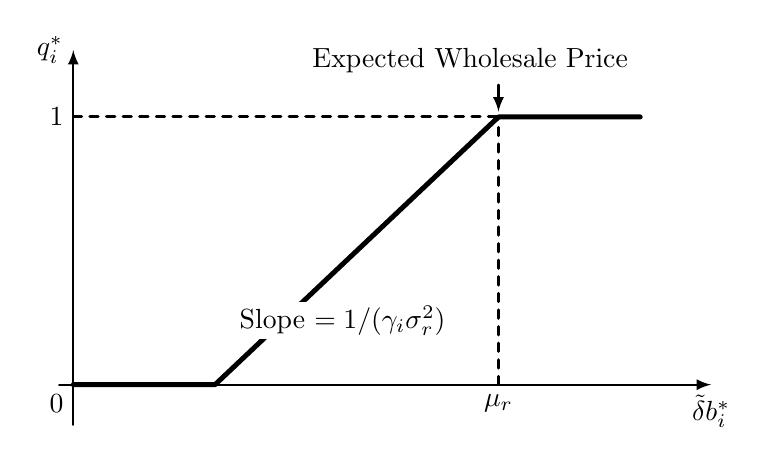
\begin{tikzpicture}[x=0.18cm,y=3.4cm,>=latex,line cap=round,line join=round]
  % Axes
  \draw[->, line width=0.8pt] (-1,0) -- (45,0) node[below] {$\tilde{\delta}b_i^\ast$};
  \draw[->, line width=0.8pt] (0,-0.15) -- (0,1.25) node[left] {$q_i^\ast$};

  % Reference lines
  \draw[dashed, line width=1.1pt] (0,1) -- (30,1);
  \draw[dashed, line width=1.1pt] (30,0) -- (30,1);

  % Portfolio rule
  \draw[line width=1.8pt] (0,0) -- (10,0) -- (30,1) -- (40,1);

  % Labels
  \node[below left] at (0,0) {$0$};
  \node[left] at (0,1) {$1$};
  \node[below] at (30,0) {$\mu_r$};

  \node[align=center] at (28,1.21) {Expected Wholesale Price};
  \draw[->, line width=0.8pt] (30,1.12) -- (30,1.02);

  \node[fill=white, inner sep=1.5pt] at (19,0.24) {Slope $= 1/(\gamma_i \sigma_r^2)$};
\end{tikzpicture}
}
\end{subfigure}
\hfill
\begin{subfigure}{0.49\textwidth}
\caption{Risk-neutral bidder employs threshold rule to shift allocation entirely}
\label{fig:portfolioneutral}
\resizebox{\textwidth}{!}{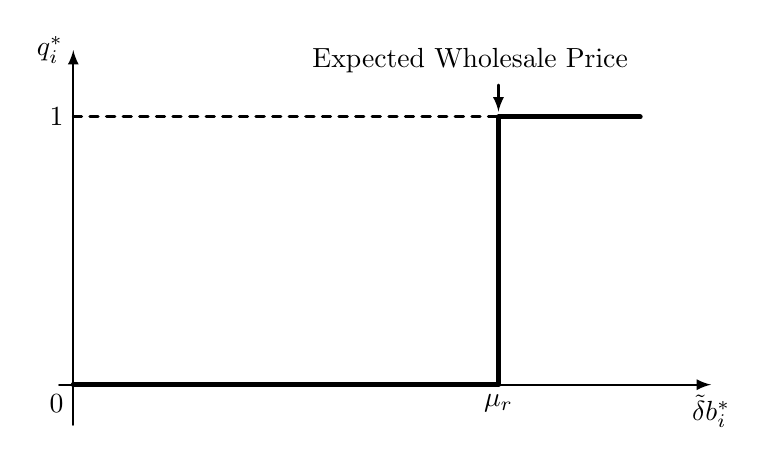
\begin{tikzpicture}[x=0.18cm,y=3.4cm,>=latex,line cap=round,line join=round]
  % Axes
  \draw[->, line width=0.8pt] (-1,0) -- (45,0) node[below] {$\tilde{\delta}b_i^\ast$};
  \draw[->, line width=0.8pt] (0,-0.15) -- (0,1.25) node[left] {$q_i^\ast$};

  % Reference lines
  \draw[dashed, line width=1.1pt] (0,1) -- (30,1);
  \draw[dashed, line width=1.1pt] (30,0) -- (30,1);

  % Threshold rule
  \draw[line width=1.8pt] (0,0) -- (30,0) -- (30,1) -- (40,1);

  % Labels
  \node[below left] at (0,0) {$0$};
  \node[left] at (0,1) {$1$};
  \node[below] at (30,0) {$\mu_r$};

  \node[align=center] at (28,1.21) {Expected Wholesale Price};
  \draw[->, line width=0.8pt] (30,1.12) -- (30,1.02);
\end{tikzpicture}
}
\end{subfigure}
\end{figure}

In any equilibrium, because the bid share does not affect the winning probability conditional on bid price, bidder $i$ chooses his share solely to optimize his portfolio conditional on winning.\footnote{
This observation is analogous to \citet{Bolotnyy2023}'s observation of a bidder's score being payoff-sufficient for his choice of unit bids in scaling auctions.
} The equilibrium winning probability function $W_i^\ast$ and cost $c_i$ therefore do not enter the optimal share decision. Given the discount factor $\tilde{\delta}$ and bid share bounds, this decision depends on the equilibrium bid price $b_i^\ast$, expected wholesale price $\mu_r$, wholesale market variance $\sigma_r^2$, and bidder $i$'s risk aversion $\gamma_i$. This separation is crucial for using bidders' bid share and price decisions separately in identification and estimation.

Bidder $i$'s optimal bid price $b_i^\ast$ satisfies
\begin{align}
\label{eq:optbsb}
\underbrace{q_i^\ast \tilde{\delta} b_i^\ast + (1 - q_i^\ast)\mu_r}_{\substack{\text{Expected revenue}}} 
= c_i 
+ \underbrace{(1-q_i^\ast)^2 \cdot \frac{\gamma_i \sigma_r^2}{2}}_{\substack{\text{Risk premium}}} 
+ \underbrace{\frac{1}{\gamma_i} \ln \left(-\frac{\gamma_i q_i^\ast \tilde{\delta} W_i^\ast(b_i^\ast)}{dW_i^\ast(b_i^\ast)/d b} + 1 \right)}_{\substack{\text{Markup}}}.
\end{align}
The two terms on the left-hand side, the purchase agreement and expected wholesale market revenues, comprise the bidder's expected revenue. The bidder optimizes the bid price by balancing the expected revenue with the three terms on the right-hand side: cost, risk premium, and markup. The markup decreases with the bidder's risk aversion coefficient $\gamma_i$ because more risk-averse bidders cut markups for fear of the possibility of losing the auction. Additionally, bidders collect higher markup when the auction is less competitive since their winning probabilities decrease little by increasing their bid prices. The equality converges to $b_i^\ast = c_i/\tilde{\delta} - W_i^\ast(b_i^\ast)/(dW_i^\ast(b_i^\ast)/d b)$ as the bidders become risk-neutral ($\gamma_i \to 0$ and $q_i^\ast \to 1$), coinciding with the standard optimal bid price formula for risk-neutral bidders \citep[e.g.,][]{Athey2007}.


\subsection{Descending-Clock Auctions}
\label{sec:dc}

I analyze descending-clock auctions in line with \citet{Milgrom1982}'s English auction model. Institutionally, these auctions are implemented as a discrete descending-clock, pay-as-bid procedure, but, for tractability, I treat them as the continuous-clock limit in which the outcome is equivalent to a uniform-price auction: bidders choose a cutoff---the lowest price they are willing to accept---as their ``bid price'' $b_i$, and winners would be paid a common clearing price pinned down at the margin, i.e., $p_i=p\coloneqq b_{M+1:N}$, where $M$ is the number of winners and $b_{M+1:N}$ denotes the $(M+1)$th lowest of $N$ bid prices.\footnote{
In the actual discrete-clock implementation, winners' final submitted prices may not coincide, and the equality $p_i=p$ may not hold exactly because bids adjust in discrete steps with a minimum decrement. I examine the robustness of this continuous-clock approximation by varying the equilibrium clearing price distribution around values implied by winners' observed final submitted prices in Section \ref{sec:results}.
}
Derivations and proofs of the statements in this section are in Online Appendix \ref{appx-sec:eqdc}.

Bidder $i$ chooses bid $(q,b)$ to maximize the expected utility of bidding:
\begin{align*}
\int \underbrace{\I(b < p)}_{\text{Winning at $p$}} \times 
\underbrace{u_i\!\left(q \tilde{\delta} p + (1 - q) \mu_r - c_i - RP_r(1-q \mid \gamma_i) \right)}_{\text{Normalized expected utility conditional on winning at $p$}} f_p(p)\, dp.
\end{align*}
The bidder takes expectation of what he expects to earn over the clearing price $p$. A pure-strategy BNE is a profile of type-contingent bid strategies under which every bidder maximizes expected utility given the equilibrium clearing price distribution $f_{p^\ast}$, where $p^\ast$ is the $(M+1)$th order statistic of $N$ equilibrium bid prices, i.e., $p^\ast \coloneqq b_{M+1:N}^\ast$. To keep the equilibrium analysis tractable, I assume $f_{p^\ast}$ is normally distributed, $\mathcal{N}(\mu_{p^\ast},\sigma_{p^\ast}^2)$, and independent of the wholesale price $r$.\footnote{
Independence is reasonable if the main drivers of the clearing price and wholesale prices differ: clearing prices move with the distribution of wind-project costs, while Brazil's wholesale price uncertainty is primarily driven by marginal hydroelectric and thermal fuel costs.
} Under an additional condition that I detail in Online Appendix \ref{appx-sec:eqdc}, by \citet{Reny2011}, a monotone pure-strategy BNE exists, and a symmetric monotone pure-strategy BNE exists when bidders are \textit{ex-ante} symmetric.

Bidder $i$'s optimal bid share satisfies $q_i^\ast = \min \left\{\max \left\{\underline{q},\ q^{\ast\ast}(b_i^\ast \mid \gamma_i) \right\},\ 1 \right\}$, where $q^{\ast\ast}(b \mid \gamma_i)$ is an unconstrained optimal bid share function implicitly defined as the solution to
\begin{align}
\label{eq:focqdc}
q^{\ast\ast} 
= \left( \frac{1}{1 + \tilde{\delta}^2 \sigma_{p^\ast}^2/\sigma_r^2} \right) 
\left( 1 - \frac{\mu_r - \tilde{\delta}\, \tilde{\mu}_{p^\ast}(q^{\ast\ast},b \mid \gamma_i)}{\gamma_i \sigma_r^2} \right).
\end{align}
$\tilde{\mu}_{p^\ast}(q,b \mid \gamma_i)$ is the effective expected equilibrium clearing price for choosing bid $(q,b)$ given risk aversion $\gamma_i$, $\tilde{\mu}_{p^\ast}(q,b \mid \gamma_i)= \mu_{p^\ast} + \sigma_{p^\ast}\, \Lambda ((\mu_{p^\ast} - b)/\sigma_{p^\ast} - q\, \gamma_i \tilde{\delta}\, \sigma_{p^\ast} )$, where $\Lambda$ is the inverse Mills ratio for a standard normal. For a risk-neutral bidder ($\gamma_i \to 0$), $\tilde{\mu}_{p^\ast}$ is the mean of the equilibrium clearing price distribution truncated from below at $b$. A risk-averse bidder effectively moves up the truncation point to $b + q \gamma_i \tilde{\delta} \sigma_{p^\ast}^2$ because he appreciates the truncation more than the risk-neutral bidder, as it reduces the risk of getting the purchase agreement at a low price. Bidder $i$'s optimal bid price makes his expected utility conditional on winning equal to zero.

I highlight several features of the optimal bid share decision. First, the equilibrium bid share $q_i^\ast$ continuously increases with the equilibrium bid price $b_i^\ast$ as in sealed-bid auctions in Figure \ref{fig:portfolioaverse}, though the relationship is now nonlinear. Second, a large equilibrium clearing price variance $\sigma_{p^\ast}^2$ has two counteracting effects. It lowers $q_i^\ast$ because the purchase agreement becomes unattractive relative to the wholesale market (channel through the term $\tilde{\delta}^2 \sigma_{p^\ast}^2/\sigma_r^2$ in equation~\eqref{eq:focqdc}). On the other hand, the effective expected equilibrium clearing price $\tilde{\mu}_{p^\ast}$ can increase because of the truncation. Third, the effect of the risk aversion coefficient $\gamma_i$ is unclear because both purchase agreement and wholesale prices are uncertain at the time of bidding. Intuitively, the risk from the clearing price uncertainty becomes more salient than the risk of the wholesale market when the bidder puts most of his electricity into the purchase agreement, which makes more risk-averse bidders move away from the purchase agreement once the bid share gets close enough to 1.


\section{Econometric Model}
\label{sec:econometric}

I present my identification results and then specialize the structural model for estimation using Brazil's new wind energy auctions. To simplify notation throughout this section, I present the model for a single, representative auction and omit auction subscripts. Heterogeneity across auctions is accounted for via observed covariates and auction fixed effects in the estimation.

\subsection{Identification}
\label{sec:identification}

I observe the joint distribution of winners' bid shares, bid prices, and capacities, where winners are selected by ranking bid prices. The challenge is to recover the joint participant distribution of equilibrium bids and capacities, $f_{q^\ast,b^\ast,C}$, from this winner distribution. I assume that $(q_i^\ast,b_i^\ast,Capacity_i)$, $i=1,\dots,N$, are independently drawn from $f_{q^\ast,b^\ast,C}$, as implied by \textit{ex-ante} symmetric bidders following a symmetric equilibrium strategy. Arranging bid prices in ascending order gives the order statistics $b_{1:N}^\ast\leq\cdots\leq b_{N:N}^\ast$; the bid shares and capacities paired with them, $q_{[1:N]}^\ast,\dots,q_{[N:N]}^\ast$ and $Capacity_{[1:N]},\dots,Capacity_{[N:N]}$, are their \textit{concomitants} \citep{Yang1977}. I extend \citet{Athey2002}'s recovery of the one-dimensional participant bid distribution from winning bids to multidimensional bids and bidder attributes. I build on the statistics literature of concomitants to connect the joint distribution of concomitants and order statistics to the original distribution from which they are drawn. In particular, under i.i.d.\ draws, the conditional distribution of a concomitant given its paired order statistic equals the original conditional distribution, $f_{Y_{[k:N]}|X_{k:N}}=f_{Y|X}$ \citep{Yang1977}. Intuitively, sorting observations by one component preserves its pairing with all remaining components.

I identify the joint distribution of bidders' risk aversion coefficients $\gamma_i $ and costs $c_i $. I also identify the expected wholesale price $\mu_r $ in sealed-bid auctions. I assume that the number of participants $N$, the distribution of procurement capacity $D$, and the wholesale market variance $\sigma_r^2$ at the time of the auction are observed for each auction. The discount factor $\delta$ is prespecified.

\textbf{Sealed-Bid Auctions.} I observe the joint distribution of the pairs of concomitants and order statistics, $f_{q_{[k:N]}^\ast,b_{k:N}^\ast,C_{[k:N]}} $, for winners, $k=1,\dots,M $, where $1 \leq M \leq N$ is the number of winners. I identify the original distribution as
\begin{align*}
f_{q^\ast,b^\ast,C} = f_{q^\ast,C|b^\ast} f_{b^\ast} = f_{q_{[k:N]}^\ast,C_{[k:N]}|b_{k:N}^\ast} f_{b^\ast}
\end{align*}
since there is a one-to-one relationship between $f_{b^\ast} $ and $f_{b_{k:N}^\ast} $ when the draws are i.i.d. \citep{Athey2002}, and $f_{q_{[k:N]}^\ast,C_{[k:N]}|b_{k:N}^\ast} $ and $f_{b_{k:N}^\ast} $ are observed for any $k$ up to $M$.

Bidders allocate all production to the risk-free purchase agreement when their discounted bid price $\tilde{\delta} b_i^\ast $ is at least as high as the expected wholesale price $\mu_r $, regardless of their types. Thus, the bids with a 100\% bid share identify $\mu_r $ as the lowest bid price at which a 100\% bid share occurs: $\mu_r = \tilde{\delta} \cdot \inf\left\{b:\Pr(q^\ast=1\mid b)>0\right\} $. Once I have $\mu_r $, I can pin down $\gamma_i $ of those who bid $q_i^\ast $ in the interior of the possible bid share $[\underline{q},1]$ by their optimal bid share decisions (equation~\eqref{eq:optqsb}) because $c_i$ does not affect the share decision conditional on $b_i^\ast $. I then recover $c_i$ using the solution to the optimal bid price decision (equation~\eqref{eq:optbsb}) with $\mu_r $ and $\gamma_i $, as \citet*{Guerre2000}, by calculating the equilibrium winning probability function using $f_{q^\ast,b^\ast,C}$.

Note that the types $(\gamma_i,c_i) $ are point identified only for those who bid $q_i^\ast $ in the interior of $[\underline{q},1]$. Any $\gamma_i > 0 $ can justify the bid share of 100\%, and the bid share of $\underline{q}$ only provides an upper bound for $\gamma_i $. Because these boundary shares do not point identify $\gamma_i$, I impose parametric assumptions on $f_\gamma$ to recover the risk aversion distribution for all participants. Once $f_\gamma$ is identified, I can point identify the distribution of $c_i $ as well.
% % Bound analysis
% Alternatively, I can evaluate the lower bound on the bidders' total wholesale market risk premium, which is a relevant measure for the policymaker, by setting the risk premiums of those with unidentified $\gamma_i $ to zero. Somewhat surprisingly, $c_i $ is partially identified without the identification of $\gamma_i $ because the markup term in the optimal bid price decision is bounded as
% \begin{align*}
% 0 < \frac{1}{\gamma_i} \ln \left(-\frac{\gamma_i \tilde{\delta} W_i^\ast(b_i^\ast)}{dW_i^\ast(b_i^\ast)/d b} + 1 \right) < -\frac{\tilde{\delta} W_i^\ast(b_i^\ast)}{dW_i^\ast(b_i^\ast)/d b} \text{ for } \gamma_i \in (0,\infty),
% \end{align*}
% and this can be narrowed down by an upper bound on $\gamma_i $ for those bidding $\underline{q}$ share.

\textbf{Descending-Clock Auctions.} I observe the joint distribution of the winners' concomitants and the lowest order statistics among the losers, $f_{Y_{[1:N]},\dots,Y_{[M:N]},b_{M+1:N}^\ast} $, where $Y_{[k:N]} = (q_{[k:N]}^\ast, C_{[k:N]}) $.\footnote{To be precise, I do not observe the ordering of the winners' concomitants because the winners' equilibrium bid prices are unobserved. The identification argument does not require this ordering because it evaluates the joint density at $y_1=\cdots=y_M=y$, which is invariant to permutations of the winners. Observing the ordering could nevertheless improve estimation efficiency by sharpening inference about each winner's latent bid price.} $b_{M+1:N}^\ast$ is observed as the equilibrium clearing price $p^\ast $. As in sealed-bid auctions, the key is to identify the conditional distribution $f_{Y|b^\ast}$ from the observed joint distribution since $f_{b^\ast}$ is identified from the order statistic distribution I observe, $f_{b_{M+1:N}^\ast} $. The observed joint distribution can be expressed using the conditional distribution as follows \citep{Yang1977}:
\begin{align}
\label{eq:identificationdc}
&f_{Y_{[1:N]},\dots,Y_{[M:N]}|b_{M+1:N}^\ast}(y_1,\dots,y_M|b_{M+1}) = \nonumber\\
& \int^{b_{M+1}} \cdots \int^{b_2} \prod_{k=1}^M f_{Y_{[k:N]}|b_{k:N}^\ast}(y_k|b_k) f_{b_{1:N}^\ast,\dots,b_{M:N}^\ast|b_{M+1:N}^\ast}(b_1,\dots,b_M|b_{M+1}) d(b_1,\dots,b_M).
\end{align}
Since $f_{Y_{[k:N]}|b_{k:N}^\ast} = f_{Y|b^\ast} $ for all $k = 1,\dots,M $, and the joint distribution of the order statistics $f_{b_{1:N}^\ast,\dots,b_{M:N}^\ast|b_{M+1:N}^\ast} $ can be calculated from $f_{b^\ast}$, the structure of the identification problem becomes similar to nonparametric instrumental variable models \citep{Newey2003}. Following that literature, I impose bounded completeness on the adjacent conditional order statistic distributions. In Appendix \ref{sec:identificationdc}, I show that this condition identifies \(f_{Y|b^\ast}\) within the class of bounded conditional densities that are positive over a common interval of bid prices. Bounded completeness admits very general families of distributions, and its sufficient conditions and testing procedures are extensively discussed (e.g.,\citealp*{Blundell2007}; \citealp{Hu2008}; \citealp{Freyberger2017}).

I cannot identify the expected wholesale price $\mu_r $ as in sealed-bid auctions since the bidders' risk aversion type $\gamma_i $ always affects their optimal bid share decision (equation~\eqref{eq:focqdc}), because both the purchase agreement and the wholesale prices are uncertain at the time of bidding. Thus, I treat $\mu_r $ as known when identifying the descending-clock model. In the empirical application, I extrapolate $\mu_r $ using the parameterization estimated from sealed-bid auctions.

I can then identify $f_\gamma$ from bidders' bid share decisions, together with the observed clearing price distribution $f_{p^\ast}$. Because winners' bid prices $b_i^\ast$ are unobserved in descending-clock auctions, I cannot identify each bidder's $\gamma_i$ from a single observed share choice. Instead, identification of $f_\gamma$ uses (i) the model-implied mapping from $(b_i^\ast,\gamma_i)$ to $q_i^\ast$ (equation~\eqref{eq:focqdc}) and (ii) the implied distribution of winners' latent bid prices $b_i^\ast$ conditional on the observed clearing price $p^\ast$, i.e., $f_{b^\ast \mid (b^\ast < p^\ast)}$. Variation in observed bid shares across auctions with different clearing price realizations, together with this truncation relationship, disciplines $f_\gamma$. Once $f_\gamma$ is identified, I can identify the distribution of $c_i$ by combining the equilibrium relationship that $b_i^\ast$ is a cutoff at which his expected utility from winning is zero and $f_{b^\ast \mid (b^\ast < p^\ast)}$.

\subsection{Estimation}
\label{sec:estimation}

The estimation procedure applies the optimal bid share and price decisions sequentially. I first use the solution to the bid share decision, equivalent to the portfolio optimization, to estimate the distribution of the risk aversion coefficient $\gamma_i $, $f_\gamma $, and the expected wholesale price $\mu_r $. I then infer the distribution of the cost types $c_i$, $f_c $, using the solution to the bid price optimization problem. I do not estimate $f_c $ in descending-clock auctions because I observe only \input{snt/auction_N_dc} clearing prices rather than individual equilibrium bid prices. I assume symmetric bidders because I only observe winners' bids, as discussed in Section \ref{sec:identification}.

To take the model to the data, I accommodate the project-specific effective bid share bounds induced by the discrete bid quantity rules. The auction rules require bid quantities to be submitted in discrete units (integers in the first auction in 2009, and up to the first decimal place in subsequent ones). Because project capacities are not always perfectly divisible by these units, the nominal lower and upper bounds on bid shares ($\underline{q}$ and $1$) are not always exactly attainable. Therefore, for each project, I calculate the effective lower and upper bounds, $\underline{q}_i$ and $\bar{q}_i$, based on the project's capacity and the auction's discrete unit. I maintain the following assumption for estimation, which incorporates these effective bounds:
\begin{assumption}
\label{assu:obsq}
The optimal bid share, evaluated at the equilibrium bid price $b_i^\ast $, is observed as a censored normal model with the unconstrained optimal bid share function $q^{\ast\ast}$ (defined in equations \eqref{eq:optqsb} and \eqref{eq:focqdc} for sealed-bid and descending-clock auctions, respectively), i.e.,
\begin{align*}
q_i^d = \min \left\{\max \left\{\underline{q}_i, q^{\ast\ast}(b_i^\ast \mid \gamma_i) + \eta_i \right\}, \bar{q}_i \right\}, \eta_i \sim \mathcal{N}(0,\sigma_\eta^2),
\end{align*}
where $q_i^d$ is the observed bid share, and $\eta_i $ is a bid share shock that is independent across bidders and auctions.
\end{assumption}
\citet{Bolotnyy2023} also make a similar assumption in their scaling auction model estimation, but without a parametric assumption on the exogenous shock. In my case, the parametric assumption of the bid share shock $\eta_i $ deals with the censoring nature of the bid share. Further details about the estimation procedures are in Online Appendix \ref{appx-sec:estimationprocedure}.

\textbf{Prespecified Parameters.} I prespecify the wholesale market variance $\sigma_r^2 $. I estimate a mean reverting process of annual wholesale prices using time-series data of spot prices. I then calculate each auction's $\sigma_r^2 $ with the future wholesale prices $r_t $ following the estimated mean reverting process.

I also prespecify descending-clock auctions' equilibrium clearing price distributions $f_{p^\ast} = \mathcal{N}(\mu_{p^\ast},\sigma_{p^\ast}^2) $. Although Section \ref{sec:identification} shows the identification of $f_{p^\ast}$, I do not estimate it because I only observe \input{snt/auction_N_dc} clearing prices. I model the equilibrium clearing price distribution conditional on the procurement capacity $D$, $f_{p^\ast|D} $, with auction covariates, including auction date, lead time, forecasted marginal cost of electricity at the time of auction, and number of participants. I then integrate it out by the procurement capacity distribution $f_D $ below to obtain $f_{p^\ast} $ because $D$ is not disclosed at the time of bidding. I prespecify the parameters in $f_{p^\ast|D} $ to those that maximize the likelihood of the observed clearing prices and $D$.

I model $f_D $ with auction covariates and prespecify the parameters to maximize the likelihood of the observed $D$, separately for sealed-bid and descending-clock auctions. $f_D $ for sealed-bid auctions is used to calculate the winning probability function in the second step of estimation. $f_D $ for descending-clock auctions is used to obtain the equilibrium clearing price distribution $f_{p^\ast} $. Prespecified parameter values are summarized in Tables \ref{appx-tab:spotestimates} and \ref{appx-tab:prespecdist} in Online Appendix \ref{appx-sec:suppstructural}. The annual discount factor $\delta$ is prespecified to be $0.95 $. I check the sensitivity of my structural estimates to the scale of the shock in the wholesale price mean reverting process, the mean and variance $(\mu_{p^\ast},\sigma_{p^\ast}^2)$ of the clearing price distribution, and the discount factor $\delta$ in Section \ref{sec:results}.

\textbf{First Step.} I estimate the risk aversion distribution $f_\gamma$, the expected wholesale price $\mu_r$, and the bid share shock variance $\sigma_\eta^2$ using the generalized method of moments. I match the probabilities of bidding at the lower and upper bid-share bounds and the conditional mean among interior bid shares in the data to those implied by Assumption \ref{assu:obsq}. I allow heterogeneous risk aversion according to $\gamma_i = \exp\left\{\alpha_{\gamma 0} + \alpha_{\gamma 1}\log(1+K_i)\right\}$, where $K_i$ is the prior started wind capacity of project $i$'s affiliated firm, as defined in Section \ref{sec:data}. This parameterization allows a firm's prior wind portfolio to affect a project's portfolio choice through its risk attitude.

I specify $\mu_r = \delta^{l} (\alpha_{r 0} + \alpha_{r 1} m) $, where $l$ is the lead time and $m$ is forecasted marginal cost of electricity at the time of auction. I include $m$ to capture time variation in bidders' expected wholesale prices. The descriptive regressions in Table \ref{tab:preliminary_regression} show that $m$ is negatively associated with bid shares, which is consistent with interpreting $m$ as a proxy for more favorable wholesale-market conditions: when wholesale prices are expected to be higher, bidders shift exposure toward the wholesale market and bid smaller shares. Additionally, the expected wholesale price is discounted according to the auction's lead time $l$. I assume $\sigma_\eta^2 $ to be the same across auctions.

In sealed-bid auctions, I use observed bid prices, assuming they are equilibrium bid prices, to compute the individual moments. In contrast, for each winner in descending-clock auctions, I numerically integrate out the winner's latent equilibrium bid price $b_i^\ast$ over the equilibrium bid price distribution conditional on being below the observed final bid price $b_i^d$, $f_{b^\ast \mid (b^\ast \leq b_i^d)}$. This conditional distribution is calculated from the equilibrium clearing price distribution $f_{p^\ast}$ using the one-to-one relationship between $f_{b^\ast}$ and $f_{p^\ast} = f_{b_{M + 1:N}^\ast}$.

\textbf{Second Step.} I estimate the cost distribution $f_c$ in sealed-bid auctions. To evaluate the winning probability and invert bids into costs, I recover the participants' joint distribution of $(\gamma_i,Capacity_i,b_i^\ast) $ from winners' bids and attributes, following the order-statistics and concomitants arguments in Section \ref{sec:identification}. First, I estimate $f_{b^\ast} $ from winners' bid prices using a pseudo-likelihood that combines their marginal order-statistic densities. $f_{b^\ast} $ is assumed to be normally distributed with auction-specific mean and common variance across auctions.

Second, I recover the conditional capacity distribution $f_{C|b^\ast}$ from winners, which is justified by the property of concomitants: under i.i.d.\ draws, the conditional distribution of a concomitant given its paired order statistic equals the original conditional distribution. So, the conditional distribution of winners' capacities given their bid prices equals that of participants. $f_{C|b^\ast}$ is assumed to be log-normally distributed with the mean parameterized by $b_i^\ast$ and auction fixed effects, and common variance across auctions. Third, I recover the conditional distribution of prior started wind capacity, $f_{K|C,b^\ast}$, using a censored normal model whose latent mean is parameterized by $Capacity_i$, $b_i^\ast$, and auction fixed effects. Combining these estimates gives $f_{K,C,b^\ast}=f_{K|C,b^\ast}f_{C|b^\ast}f_{b^\ast}$. Given the first-step parameterization of the deterministic relationship between $\gamma_i$ and $K_i$, this joint distribution directly implies $f_{\gamma,C,b^\ast}$.

I next compute the sealed-bid auction's equilibrium winning probability functions $W_i^\ast $ using $f_{\gamma,C,b^\ast}$. $W_i^\ast $ is symmetric for symmetric bidders, i.e., $W_i^\ast = W^\ast $ for all $i$. $f_{\gamma,C,b^\ast}$ implies $f_{C,q^\ast,b^\ast}$ because $b_i^\ast $ uniquely determines the equilibrium bid share $q_i^\ast $ as the solution to the bid share decision conditional on $\gamma_i $. Conditional on auction covariates, I assume that the realized procurement capacity $D$ is independent of participants' bids and capacities. I then simulate $W^\ast(b) $ according to equation~\eqref{eq:winprob} using $f_{C,q^\ast,b^\ast}$ and $f_D$.

I finally infer the winners' costs $c_i $ from their observed bids and estimated $\gamma_i $ using the solution to the bid price decision in equation~\eqref{eq:optbsb}. I also recover the participants' joint distribution of $\gamma_i $ and $c_i $ from the estimated $f_{\gamma,C,q^\ast,b^\ast} $ by simulation.

\section{Structural Estimates}
\label{sec:results}

I first estimate the bidders' risk aversion and expected wholesale prices from bid share decisions using all \input{snt/auction_N_sb} sealed-bid and \input{snt/auction_N_dc} descending-clock auctions from \input{snt/auction_year_min} to \input{snt/auction_year_max}. I then recover the bidders' cost distribution using the \input{snt/auction_N_sb_nomissing} sealed-bid auctions from \input{snt/auction_year_min_sb} to \input{snt/auction_year_max_sb} for which the number of participants is observed.

Table \ref{tab:first_stage_estimates} shows estimates for the risk aversion parameters $\alpha_\gamma $ and expected wholesale price parameters $\alpha_r$. The implied capacity weighted average risk aversion coefficient among winners is \input{snt/gamma_mean_winner_all} across the \input{snt/auction_N} auctions. For a bidder with $\gamma_i = \input{snt/gamma_mean_winner_all}$, the certainty equivalent of a 50--50 lottery paying \$\input{snt/lottery_low}/MWh or \$\input{snt/lottery_high}/MWh is \$\input{snt/gamma_mean_winner_all_lotteryce}/MWh, compared with an expected price of \$\input{snt/lottery_mean}/MWh, indicating substantial risk aversion.

The risk aversion coefficient should nevertheless be interpreted with caution because its estimate depends heavily on the prespecified wholesale market variance $\sigma_r^2 $. By contrast, the implied risk premium is robust to misspecification of $\sigma_r^2 $, as shown in Table \ref{appx-tab:sa_rp_cost} in Online Appendix \ref{appx-sec:suppstructural}. If the true $\sigma_r^2 $ were larger, the estimated $\gamma_i $ would fall in inverse proportion, leaving the risk premium $RP_r(1|\gamma_i) = \gamma_i \sigma_r^2/2 $ unchanged but moving the certainty equivalent of the illustrative lottery closer to its expected value.

\begin{table}[htb!]
\caption{First-stage structural parameter estimates from bid share decisions}
\label{tab:first_stage_estimates}
\centering
\input{table/first_stage_estimates}
\tabnote[\textwidth]{Notes: The parameters are estimated using all \input{snt/bidder_N} winning bids in \input{snt/auction_N_sb} sealed-bid and \input{snt/auction_N_dc} descending-clock auctions from \input{snt/auction_year_min} to \input{snt/auction_year_max}. Prior started wind capacity is the cumulative capacity of the affiliated firm's previously awarded wind projects whose contractual delivery periods had begun by the time of the auction. The forecasted marginal cost of electricity is the average of the 6th to 10th years of the ten-year forecasts of the marginal cost of operation of the Brazilian power system (Custo Marginal de Opera\c{c}\~ao) at the time of the auction, collected from EPE's Ten-Year Energy Expansion Plan \citep{EPE2026}. Standard errors (in parentheses) are calculated using \input{snt/bs_num} bootstrap replications that resample firms globally.}
\end{table}

The negative prior started wind capacity coefficient suggests that moving from no prior started wind capacity to 100 MW is associated with a \input{snt/gamma_prior_capacity_100mw_decline_pct} lower risk aversion coefficient, although the coefficient is imprecisely estimated. Projects affiliated with firms with larger prior wind portfolios appear less risk averse and are willing to take on more wholesale market risk to increase expected profits by bidding lower shares.

The implied expected wholesale prices range from \$\input{snt/exp_wholesale_price_min}/MWh to \$\input{snt/exp_wholesale_price_max}/MWh across all auctions from \input{snt/auction_year_min} to \input{snt/auction_year_max}. These expected wholesale prices are comparable to the average spot price from \input{snt/auction_year_min} to \input{snt/spot_price_year_max}, \$\input{snt/spot_price_mean_during_auction}/MWh. The stationary mean of the estimated annual spot price process from \input{snt/spot_price_year_min} to \input{snt/spot_price_year_max}, \$\input{snt/stationary_wholesale_price}/MWh, is close to the full-sample historical average of \$\input{snt/spot_price_mean_all}/MWh but substantially below the bid-implied expectations. This difference underscores the importance of estimating expected wholesale prices from bids.

The forecasted marginal cost coefficient $\alpha_{r1}$ is relatively close to one, consistent with the long-term forecast capturing bidders' beliefs about future market conditions. One interpretation of the coefficient below one is that investors anchor on a baseline expectation and only partially incorporate long-term forecasts, which cover years 6 through 10 from the time of the auction. The approach of estimating expected wholesale prices directly from the bid data circumvents the challenges of relying on external forecasts as direct proxies for bidders' expectations. Figure \ref{appx-fig:bidshare_gof} in Online Appendix \ref{appx-sec:suppstructural} shows that the model broadly captures the observed bid share distribution and the relationships between bid shares and purchase agreement prices, prior started wind capacity, and forecasted marginal cost.

Given the estimates from the first step, I estimate the winning probability functions and then infer costs from bid price decisions in \input{snt/auction_N_sb_nomissing} sealed-bid auctions. The estimated winning probability functions yield plausible winning probabilities for the observed bids (Figure \ref{appx-fig:winprob} in Online Appendix \ref{appx-sec:suppstructural} plots the predicted winning probabilities for each auction). The estimated equilibrium bid price, capacity, and prior started wind capacity distributions used to calculate the equilibrium winning probability function are summarized in Table \ref{appx-tab:winprobparam} in Online Appendix \ref{appx-sec:suppstructural}. Unless otherwise noted, the summary statistics reported below use capacity weights.

The estimated winners' average cost is \$\input{snt/cost_mean_winner}/MWh (95\% confidence interval (CI): \$\input{snt/cost_mean_winner_ci_lower}--\$\input{snt/cost_mean_winner_ci_upper}/MWh). As discussed in Section \ref{sec:model}, the cost here is effective cost, which combines physical project cost and the outside payoff. During the relevant period, however, the limited prevalence of construction outside these auctions (see Section \ref{sec:contextdata}) suggests that outside payoffs were relatively small. I therefore interpret the estimated cost approximately as physical project cost. The winners' average markup is \$\input{snt/markup_mean_winner}/MWh (95\% CI: \$\input{snt/markup_mean_winner_ci_lower}--\$\input{snt/markup_mean_winner_ci_upper}/MWh).

Winners' risk premiums from selling all electricity in the wholesale market average \$\input{snt/rp_mean_winner}/MWh, or \input{snt/rp_cost_ratio_mean_winner} of their average cost. The 95\% CI is \$\input{snt/rp_mean_winner_ci_lower}--\$\input{snt/rp_mean_winner_ci_upper}/MWh. For the \input{snt/bidder_N_sb_nomissing} winners included in the cost estimation (total capacity of \input{snt/total_capacity_sb_nomissing} GW, \input{snt/total_capacity_pct_sb_nomissing} of the overall generation capacity in Brazil in 2020 \citep{Tolmasquim2021}), these estimates imply that the winners' overall risk premium is \$\input{snt/total_rp_sb_nomissing} billion for projects with an aggregate estimated cost of \$\input{snt/total_cost_sb_nomissing} billion. In other words, to entice these investors to install projects with an aggregate estimated cost of \$\input{snt/total_cost_sb_nomissing} billion, the policymaker would save \$\input{snt/total_rp_sb_nomissing} billion by taking on all wholesale market risk using full share purchase agreements, relative to a subsidy policy that left all the risk with the investors (see Section \ref{sec:theory} for definitions of these two policy endpoints). The excess of \$\input{snt/total_rp_sb_nomissing} billion would be able to cover the additional costs of \input{snt/additional_capacity_rp_sb_nomissing} GW of wind turbines. However, the risks are substantial: the expected wholesale price estimates and the prespecified wholesale price process imply aggregate discounted revenue of \$\input{snt/total_wholesale_revenue_mean_sb_nomissing} billion with a standard deviation of \$\input{snt/total_wholesale_revenue_sd_sb_nomissing} billion from these projects over 20 years.

The policymaker may assess the scale of this exposure by considering the burden if aggregate net expenditure is passed through uniformly across all electricity consumers. Using Brazil's 2019 residential consumption, customer counts, and tariffs \citep{EPE2021}, the subsidy policy would increase the average residential monthly bill of \$\input{snt/residential_monthly_bill_2019} by \input{snt/subsidy_monthly_surcharge_cent} cents. A full share purchase agreement would instead reduce the expected monthly bill by \input{snt/fullpa_monthly_bill_reduction_cent} cents, but its wholesale market exposure would have a monthly bill equivalent standard deviation of \input{snt/fullpa_monthly_bill_sd_cent} cents, or \input{snt/fullpa_monthly_bill_sd_pct} of the average bill.

I next recover the participant distribution that provides the baseline for the counterfactual analysis. Table \ref{tab:gamma_cost_dist} summarizes the participants' joint distribution of the risk aversion coefficient $\gamma_i $ and cost $c_i $ within each of the \input{snt/auction_N_sb_nomissing} sealed-bid auctions used in the cost estimation. The average participant's $\gamma_i $ is comparable to the average winner's. The participant standard deviation (SD) of $\gamma_i$, \input{snt/gamma_sd_participant}, implies that, for the same wholesale market exposure, an investor 1 SD above the average has a risk premium \input{snt/gamma_1sd_ratio} times that of an investor 1 SD below the average. The average participant has a cost that is \$\input{snt/cost_diff_participant_winner}/MWh (corresponding to \input{snt/cost_diff_within_auction_sd_ratio} participant cost SDs) higher than the average winner's. The cost estimates are in a reasonable range compared to the engineering estimates.\footnote{
	EPE's engineering cost estimates imply that the participants' cost distribution has a mean and SD of \$\input{snt/engineering_cost_mean}/MWh and \$\input{snt/engineering_cost_sd}/MWh, respectively, from \input{snt/engineering_cost_year_min} to \input{snt/auction_year_max_sb} \citep{EPE2022b}. This engineering cost mean is close to but lower than my estimated mean cost of \$\input{snt/cost_mean_participant_post2010}/MWh, averaged over the same period (\input{snt/engineering_cost_year_min}--\input{snt/auction_year_max_sb}). My revealed preference estimates may exceed engineering costs because the estimated cost includes outside payoffs and may also include friction costs unrelated to wholesale market risk.
}
The correlation between $\gamma_i $ and $c_i $ is imprecisely estimated around zero. A linear projection of participants' cost distribution also yields a reasonable cost trend and lead time effect, as summarized in Figure \ref{appx-fig:c_dist_lp} in Online Appendix \ref{appx-sec:suppstructural}.

% EPE's cost estimate details
% (author calculation based on the government's fixed and variable cost estimates, assuming the same discount factor $\delta = 0.95 $ and the loan at the base interest rate)

\begin{table}[htb!]
\caption{Within-auction joint distribution of risk aversion coefficient $\gamma_i$ and cost $c_i$}
\label{tab:gamma_cost_dist}
\centering
\input{table/gamma_cost_dist}
\tabnote[\textwidth]{Notes: The joint distribution is estimated using the \input{snt/auction_N_sb_nomissing} sealed-bid auctions for which the number of participants and participants' total capacity are observed from \input{snt/auction_year_min_sb} to \input{snt/auction_year_max_sb}. The reported moments are calculated within each auction and then averaged across auctions using participants' total capacity as weights. 95\% confidence intervals (CIs) are in brackets, calculated using \input{snt/bs_num} bootstrap replications that resample firms globally.}
\end{table}

% sensitivity analysis
Because sealed-bid bidders choose shares and prices jointly, their portfolio choice condition links observed choices directly to risk premiums, making the risk premium estimates insensitive to the prespecified wholesale price volatility. In contrast, in descending-clock auctions, bidders choose shares before the purchase agreement price is known, making their portfolio choices more dependent on the prespecified wholesale price volatility and clearing price distribution. Table \ref{appx-tab:sa_rp_cost} in Online Appendix \ref{appx-sec:suppstructural} reports that winners' average risk premium remains within \$\input{snt/sa_rp_panels_abc_min}--\$\input{snt/sa_rp_panels_abc_max}/MWh and their average cost within \$\input{snt/sa_cost_panels_abc_min}--\$\input{snt/sa_cost_panels_abc_max}/MWh across a wide range of wholesale price volatility and clearing price distribution specifications. Moreover, the risk premium to cost ratio remains between \input{snt/sa_rp_cost_ratio_delta_min} and \input{snt/sa_rp_cost_ratio_delta_max} across discount factors $\delta =$ 0.90, 0.95, and 0.99, even though a different discount factor mechanically rescales discounted risk premiums and costs. Thus, counterfactual implications based on the relative cost-risk trade-off should be similar as long as investors share a common discount factor.

\section{Counterfactual Analysis}
\label{sec:counterfactuals}

Future wind technology cost declines are uncertain and difficult to forecast accurately \citep{Wiser2021}. As physical costs decline, wind power investment without policymaker support becomes viable, reducing the incremental value of support through purchase agreements. This cost uncertainty complicates the policymaker's choice of risk sharing before an auction. Risk sharing contracts, discussed in Section \ref{sec:theory}, can allow each bidder to choose its purchase agreement share or let the policymaker impose a common share on all bidders. Brazilian new energy auctions allow bidder share choice, which may automatically phase out purchase agreement support as bidders respond to privately known cost declines by reducing their shares. I compare these auctions with fixed share auctions, in which the policymaker chooses the common share $\lambda \in [0,1] $ of electricity for which she bears wholesale market sales risk, encompassing subsidies ($\lambda=0$), full share purchase agreements ($\lambda=1$), and risk sharing contracts between these extremes. The policymaker may update this fixed share across auctions as information about technology costs arrives but cannot condition it within an auction on bidders' privately known realized costs.

\subsection{Counterfactual Design and Computation}

Physical cost shifts and auction policy changes may affect the incremental value of an auction and bidders' participation decisions. I extend the sealed-bid auction model in Section \ref{sec:sb} to allow endogenous participation, in the spirit of \citet{Samuelson1985}, and calibrate the qualification cost so that the model matches the observed proportion of qualified participants among registered projects, following \citet{Bolotnyy2023}. To pin down the incremental auction value, I specify the outside payoff $\pi_{0i}$ as the maximum of zero (i.e., not building) and the certainty equivalent profit from building outside the auction and selling all electricity in the wholesale market, $\mu_r-c_i^{physical}-\gamma_i\sigma_r^2/2$. Projects with a positive outside payoff can build even if they do not participate in or win the auction.

With fixed share auctions, bidders only choose their bid prices and cannot choose their shares. I make two adjustments to the auction model in Section \ref{sec:model} to encompass subsidy ($\lambda=0$) auctions. First, winners are selected using an objective capacity $\widetilde D$ based on installed capacity rather than capacity allocated to the auction. To make the comparison between bidder share choice and fixed share auctions fair, both auction formats rank projects by bid price and make full project awards until installed capacity $\sum_i Capacity_i $ reaches the objective capacity $\widetilde D$.

Second, in fixed share auctions, bidders submit a transfer bid per MWh of total production rather than a price per MWh allocated to the purchase agreement. If bidder $i$ wins with bid $b_i$, for each period during the contract, the bidder provides $\lambda \times Capacity_i \times H$ MWh of electricity through the purchase agreement, and the auctioneer pays $b_i \times Capacity_i \times H$. At $\lambda=0$, winners sell all electricity in the wholesale market while the bid determines the generation subsidy amount. By contrast, I maintain the bid price per MWh of production allocated to the auction structure in bidder share choice auctions as in Section \ref{sec:model}. Thus, zero bid share, $q_i=0$, is an outside action rather than an auction bid: the project does not compete for auction support and builds solely for the wholesale market if doing so is viable.

I compute equilibria under physical cost reductions from zero to \$10/MWh in \$1/MWh increments, starting from the baseline participant distribution constructed from the estimates. I use one representative synthetic pay-as-bid sealed-bid auction under bidder share choice and a grid of fixed shares $\lambda$. I hold the wholesale price process fixed across these scenarios, which is a reasonable approximation because the representative auction and the associated construction remain small relative to total electricity supply.

To make equilibrium participation and bidding tractable with the two-dimensional bidder type $(\gamma_i,c_i)$, I make three simplifications. First, I consider two risk aversion types, low and high, rather than a continuous distribution.\footnote{
In principle, the computational approach could extend to any finite number of risk aversion types using the same joint differential system under the common upper support restriction.
} I construct the baseline participant joint distribution of $(\gamma_i,c_i)$ to match the estimated moments with two equally weighted risk aversion types. Second, I assume that capacity is independent of $(\gamma_i,c_i)$ and follows its empirical marginal distribution, consistent with its weak estimated relationship with risk aversion and bid price. Third, I require the equilibrium participant bid price distributions for the two risk aversion types to share a common upper support $\bar b$. Within each risk type, equilibrium bid price and \emph{ex-ante} incremental auction value are monotone in cost. Thus, the common upper support implies a single bid price $\bar b$ for the marginal participants while allowing their cost cutoffs to differ by risk aversion type.\footnote{
The marginal participants' auction values deviate from the common qualification cost by at most \input{snt/cf_common_support_low_value_above_max_pct}, supporting the common upper support approximation (details in Online Appendix \ref{appx-sec:counterfactual_computation}).
}

These simplifications enable the symmetric equilibrium participation and bidding problem with two-dimensional bidder types to be formalized as a joint system of ordinary differential equations. Solving this system requires two starting values at the common upper support: $\bar b$ and $-\widetilde W^\ast(\bar b)/(d\widetilde W^\ast(\bar b)/db) $, where \(\widetilde W^\ast\) is a counterfactual equilibrium winning probability function under the objective capacity ($\widetilde D$) scheme. Conditional on these two starting values, the joint differential system determines a unique bidding path. The calibrated qualification cost imposes one restriction on the two starting values and does not uniquely determine them. I use the following continuation rule to keep equilibrium selection comparable across adjacent cost reduction scenarios. For each auction format, I solve cost reductions sequentially and, among starting values consistent with the qualification cost, select those closest to the preceding scenario's solution. Further computational details are in Online Appendix \ref{appx-sec:counterfactual_computation}.

\subsection{Counterfactual Results}

\textbf{Participation.} The participation rate barely changes across auction formats and cost scenarios, ranging from \input{snt/cf_entry_rate_min} to \input{snt/cf_entry_rate_max}, and thus the number of competitors changes little. Equilibrium bids adjust so that projects near the baseline participation margin continue to receive the incremental auction value needed to cover the fixed qualification cost.

Nonetheless, Figure \ref{fig:counterfactual_entry} shows that the participant risk aversion composition may change. Under fixed shares, the composition changes with $\lambda$ because a purchase agreement that removes wholesale market risk is more valuable to the high risk aversion type (Figure \ref{fig:counterfactual_entry_fixed}). Relative to a subsidy ($\lambda = 0$), a partial purchase agreement initially increases the high risk aversion proportion, but the marginal purchase agreement gain diminishes as $\lambda$ approaches one (a full share purchase agreement) and equilibrium bid price adjustments absorb more of the gain. At \(\lambda=1\), neither risk aversion type bears wholesale market risk conditional on winning, so the marginal purchase agreement gain becomes zero for both types and differential participation disappears in the simulated equilibrium. In contrast, under bidder share choice, the high risk aversion proportion rises slightly as costs decline because construction without auction support becomes relatively more attractive to low risk aversion bidders, while endogenous share and price adjustments largely stabilize participant composition (Figure \ref{fig:counterfactual_entry_bidder_choice}).

\begin{figure}[htb!]
\caption{High risk aversion proportion among participants}
\label{fig:counterfactual_entry}
\centering
\begin{subfigure}{0.49\textwidth}
\caption{Fixed share}
\label{fig:counterfactual_entry_fixed}
\includegraphics[width=\textwidth]{counterfactual_participant_fixed_primary.png}
\end{subfigure}
\hfill
\begin{subfigure}{0.49\textwidth}
\caption{Bidder share choice}
\label{fig:counterfactual_entry_bidder_choice}
\includegraphics[width=\textwidth]{counterfactual_participant_choice_primary.png}
\end{subfigure}
\fignote{Notes: Panel (a) reports fixed share auctions across \(\lambda\) (the share of electricity for which the policymaker bears wholesale market sales risk) at physical cost reductions of \$0/MWh, \$5/MWh, and \$10/MWh. Panel (b) reports the bidder share choice auction across physical cost reductions.}
\end{figure}

\textbf{Portfolio Adjustment.} Under bidder share choice, bidders shift their portfolio from the purchase agreement to the wholesale market as physical costs decline and construction relying solely on the wholesale market becomes viable. The capacity weighted winner mean of share $q_i$ falls from $\input{snt/cf_choice_winner_q_m0}$ to $\input{snt/cf_choice_winner_q_m5}$ after a \$5/MWh cost reduction and $\input{snt/cf_choice_winner_q_m10}$ after a \$10/MWh reduction (Figure \ref{fig:counterfactual_bidder_choice_q}). Construction without auction support begins after physical costs fall by about \$6/MWh and expands rapidly, reaching \input{snt/cf_choice_outside_capacity_m8} MW after an \$8/MWh reduction---exceeding the representative auction's expected objective capacity of \input{snt/cf_expected_objective_capacity} MW and equaling \input{snt/cf_choice_outside_capacity_participant_pct_m8} of participants' expected aggregate capacity of \input{snt/cf_expected_participant_capacity} MW---and \input{snt/cf_choice_outside_capacity_m10} MW after a \$10/MWh reduction, more than four times the objective capacity and \input{snt/cf_choice_outside_capacity_participant_pct_m10} of that expected aggregate capacity (Figure \ref{fig:counterfactual_outside_capacity}). Virtually all construction without auction support comes from auction participants who lose.

\begin{figure}[htb!]
\caption{Auction outcomes under counterfactual physical cost reductions}
\label{fig:counterfactual_selection}
\centering
\begin{subfigure}{0.49\textwidth}
\caption{Winner mean bid share}
\label{fig:counterfactual_bidder_choice_q}
\includegraphics[width=\textwidth]{counterfactual_choice_q_primary.png}
\end{subfigure}
\hfill
\begin{subfigure}{0.49\textwidth}
\caption{Capacity built without auction support}
\label{fig:counterfactual_outside_capacity}
\includegraphics[width=\textwidth]{counterfactual_outside_capacity_mechanisms.png}
\end{subfigure}
\medskip
\begin{subfigure}{0.49\textwidth}
\caption{Winner risk aversion composition}
\label{fig:counterfactual_winner_high_gamma}
\includegraphics[width=\textwidth]{counterfactual_winner_high_gamma_mechanisms.png}
\end{subfigure}
\hfill
\begin{subfigure}{0.49\textwidth}
\caption{Winner markup}
\label{fig:counterfactual_winner_markup}
\includegraphics[width=\textwidth]{counterfactual_markup_mechanisms.png}
\end{subfigure}
\fignote{Notes: Panels (a) and (b) report the bidder share choice auction only. Panels (c) and (d) compare bidder share choice with fixed shares $\lambda\in\{0,0.5,1\}$, where $\lambda$ is the share of electricity for which the policymaker bears wholesale market sales risk.}
\end{figure}

The winner risk aversion composition reflects two forces affecting incremental auction values. First, as physical costs decline and construction without auction support becomes viable, this outside opportunity is more attractive to low risk aversion bidders. Their incremental auction values therefore decline relative to those of high risk aversion bidders, raising the high risk aversion type's proportion among winners (Figure \ref{fig:counterfactual_winner_high_gamma}). Second, at a given cost reduction, a smaller fixed share $\lambda$ stabilizes a smaller portion of each winner's revenue, leaving more wholesale market risk with bidders and shifting awards toward low risk aversion bidders. Under bidder share choice, winner composition initially coincides with that under \(\lambda=1\) because winners choose full shares. As physical costs decline, bidders reduce their shares according to their individual costs and risk aversion, and winner composition moves gradually toward that under \(\lambda=0.5\) as the winner mean bid share falls toward 0.5.

Under bidder share choice, the winner markup rises from \$\input{snt/cf_choice_winner_markup_m0}/MWh to \$\input{snt/cf_choice_winner_markup_m4}/MWh after a \$4/MWh cost reduction, then falls to \$\input{snt/cf_choice_winner_markup_m10}/MWh after a \$10/MWh reduction (Figure \ref{fig:counterfactual_winner_markup}). Moderate cost reductions move bidders away from the full share purchase agreement corner ($q_i = 1$) and make bidder specific portfolio choice valuable before construction without auction support becomes viable. Winners retain part of the additional value created by portfolio flexibility as markup. Further physical cost reductions decrease the markup as construction without auction support becomes increasingly attractive, reducing the incremental auction value. Markups under fixed share formats lack the initial portfolio choice channel and are relatively flat until construction without auction support becomes viable, after which they fall.

\textbf{Policy Implications.} Policies that leave more wholesale market risk with investors favor low risk aversion projects. The correlation between cost and risk aversion can amplify or offset this selection, but the small estimated correlation does not change the qualitative pattern here. If smaller or less diversified developers are systematically more risk averse (as suggested by the negative prior started wind capacity coefficient in Table \ref{tab:first_stage_estimates}), moving from a full share purchase agreement toward a subsidy can disproportionately shift auction awards away from them. Bidder share choice moderates this distributional effect and offers a gradual, type-specific phase out of support: bidders reveal how much revenue stabilization they require through their purchase agreement shares, and projects that no longer value auction support can build without it. However, bidder share choice temporarily increases the winner markup as projects approach the point at which construction without auction support becomes viable because winners retain part of the value created by portfolio flexibility.

The preceding results show how auction format affects outcomes as physical costs decline. Whether the policymaker finds these outcomes worth the wholesale market risk she bears under each auction format depends on her own risk attitude. Following Section \ref{sec:theory}, I evaluate the policymaker's welfare using the certainty equivalent net expenditure, defined as the sum of the expected net expenditure and the policymaker's risk premium from her wholesale market exposure. I illustrate the certainty equivalent under two policymaker risk attitudes. The risk-neutral policymaker assigns a zero risk premium to any exposure. The risk-averse policymaker uses the same CARA coefficient as the average baseline participant, i.e., the policymaker's risk aversion coefficient is $\gamma_{PM}=E[\gamma_i]$.

Figure \ref{fig:counterfactual_policy} reports the certainty equivalent for the 20-year generation associated with the representative auction's objective capacity. The risk-neutral policymaker cares only about expected net expenditure and therefore prefers to take all wholesale market risk from risk-averse investors: a subsidy ($\lambda=0$) is the most costly policy, while a full share purchase agreement ($\lambda=1$) is the least costly across all physical cost reductions. The risk-averse policymaker instead prefers to divide wholesale market risk approximately equally between herself and investors, consistent with Section \ref{sec:theory}. Consequently, $\lambda=0.5$ minimizes her certainty equivalent, while $\lambda=0$ and $\lambda=1$ yield similarly higher certainty equivalents. Under bidder share choice, winners initially choose full shares, so its certainty equivalent coincides with that under $\lambda=1$. As physical costs decline, winners allocate more production to the wholesale market according to their individual costs and risk aversion, and bidder share choice approaches the $\lambda=0.5$ policy as the winner mean bid share falls toward 0.5.

\begin{figure}[htb!]
\caption{Policymaker certainty equivalent net expenditure}
\label{fig:counterfactual_policy}
\centering
\begin{subfigure}{0.49\textwidth}
\caption{Risk-neutral policymaker, $\gamma_{PM}=0$}
\includegraphics[width=\textwidth]{counterfactual_pm_ce_rn_mechanisms.png}
\end{subfigure}
\hfill
\begin{subfigure}{0.49\textwidth}
\caption{Risk-averse policymaker, $\gamma_{PM}=E[\gamma_i]$}
\includegraphics[width=\textwidth]{counterfactual_pm_ce_ra_mechanisms.png}
\end{subfigure}
\fignote{Notes: The figure reports the policymaker's certainty equivalent (CE) net expenditure, defined in Section \ref{sec:theory}, for the 20-year generation associated with the representative auction's objective capacity under bidder share choice and fixed shares $\lambda\in\{0,0.5,1\}$. $\gamma_{PM}$ is the policymaker's risk aversion coefficient. Negative values indicate that the policymaker’s expected wholesale revenue exceeds the sum of expected payments to winners and her risk premium from wholesale market exposure.}
\end{figure}

If the policymaker knew bidders' private costs and risk aversion well enough to predict the winning projects' average share before the auction, she could choose a fixed share that replicates the aggregate wholesale market risk exposure produced by bidder share choice. Bidder share choice instead adjusts her exposure through bidders' endogenous bids without requiring her to observe this private information. To quantify the cost of this decentralized adjustment, Table \ref{tab:counterfactual_policy} compares bidder share choice with a matched fixed share auction that sets $\lambda$ equal to the bidder share choice auction's capacity weighted winner mean bid share, which approximately holds the policymaker's aggregate wholesale market risk exposure fixed. The matched fixed share yields the same or lower certainty equivalent while keeping total capacity built nearly as good as bidder share choice. The difference in certainty equivalents closely follows the difference in winner markups: at a \$6/MWh cost reduction, the aggregate winner markup difference is about \$\input{snt/cf_matched_markup_gap_m6_million} million, and the certainty equivalent difference peaks at about \$\input{snt/cf_matched_ce_gap_m6_million} million for both policymakers. Bidder portfolio flexibility creates value that winners partially retain as markup. The fixed share removes this flexibility and therefore leaves less value with winners.\footnote{
This mechanism parallels \citet{Bolotnyy2023}: portfolio flexibility can insure bidders and support more aggressive bidding, but it can also let privately informed bidders retain value from optimizing the portfolio itself.
}

\begin{table}[htb!]
\caption{Matched fixed share auction comparison}
\label{tab:counterfactual_policy}
\centering
\input{table/counterfactual_policy}
\tabnote[\textwidth]{Notes: The matched fixed share auction sets $\lambda$ equal to the corresponding bidder share choice auction's capacity weighted winner mean bid share. Total capacity built includes auction winners and construction relying solely on the wholesale market. The risk-neutral policymaker has the risk aversion coefficient $\gamma_{PM}=0$, and the risk-averse policymaker has $\gamma_{PM}=E[\gamma_i]$. Policymaker certainty equivalent (CE) net expenditure and winner markup are multiplied by the 20-year generation associated with the representative auction's objective capacity. Negative CE values indicate that the policymaker’s expected wholesale revenue exceeds the sum of expected payments to winners and her risk premium from wholesale market exposure.}
\end{table}


\section{Conclusion}
\label{sec:conclusion}

This paper develops a structural auction framework to quantify the cost-risk trade-off from transferring wholesale electricity market risk between renewable investors and policymakers. Conditional on the bid price, bid shares do not affect the likelihood of winning, so bidders' share choices reveal their portfolio trade-offs between a risk-free purchase agreement and a risky wholesale market. Combining these choices with bid prices identifies investors' risk premiums and costs. I also show that winners' bids and attributes identify the joint participant distribution when the auction ranks bidders using a single bid component.

In Brazil, the average winner's wholesale market risk premium equals \input{snt/rp_cost_ratio_mean_winner} of estimated cost. For the winning projects included in the cost estimation, the aggregate risk premium is \$\input{snt/total_rp_sb_nomissing} billion relative to an aggregate estimated cost of \$\input{snt/total_cost_sb_nomissing} billion. A full share purchase agreement would reduce the policymaker's expected net expenditure by this risk premium relative to a subsidy but would transfer all wholesale market risk to the policymaker. The counterfactuals show that smaller fixed shares favor bidders with lower risk aversion, whereas bidder share choice moderates this compositional effect by allowing bidders to adjust their shares to their private types. This flexibility lets winners retain part of the value it creates as a markup. A policymaker who could predict the winning projects' average share could impose it in advance to match her aggregate wholesale market risk exposure, generally lowering winner markups and her certainty equivalent net expenditure while leaving total capacity built nearly unchanged.

Determining the preferred feasible policy ultimately requires measuring the policymaker's risk premium, including how losses are financed. A broader welfare comparison must also account for the value of public funds and the external benefits generated by additional renewable investment \citep{Hahn2026}. Another direction for future research would be to allow bid shares to affect winner selection, which could enable screening by risk aversion and extend the use of risk as a screening instrument in \citet{Maskin1984}, although the desirability of such screening would depend on the policymaker's objective. Separately identifying heterogeneity in expected-return beliefs and risk premiums remains a useful direction for future research \citep*{Egan2026}.

%%% APPENDIX %%%
\appendix
\setcounter{assumption}{0}
\renewcommand{\theassumption}{A\arabic{assumption}}
\renewcommand{\theHassumption}{A\arabic{assumption}}

\section{Identification of Descending-Clock Auctions}
\label{sec:identificationdc}

Section \ref{sec:identification} identifies $f_{b^\ast} $ from $f_{b_{M+1:N}^\ast} $, so the conditional order statistic distributions below are all identified. I restrict attention to conditional densities $f_{Y|b^\ast} $ that are bounded and positive on a common interval support. I impose the following bounded completeness condition and show that it identifies any such conditional density.
\begin{assumption}[Bounded completeness of conditional order statistic distributions]
\label{assu:complete}
For $k = 1,\dots,M $, and every bounded measurable function $h$ on the support of bid price $b^\ast $,
\begin{align*}
\int_{-\infty}^{b_{k+1}} h(b_k) f_{b_{k:N}^\ast|b_{k+1:N}^\ast}(b_k|b_{k+1}) db_k = 0 \text{ for a.e. } b_{k+1} \text{ implies } h(b_k) = 0 \text{ a.s.}
\end{align*}
\end{assumption}
\begin{proof}[Identification]
I can transform the joint distribution of the order statistics into a sequence of conditional distributions using the Markov property of order statistics \citep*[e.g.,][]{Arnold2008}:
\begin{align}
\label{eq:markov}
f_{b_{1:N}^\ast,\dots,b_{M:N}^\ast|b_{M+1:N}^\ast} &= f_{b_{1:N}^\ast,\dots,b_{M-1:N}^\ast|b_{M:N}^\ast,b_{M+1:N}^\ast} f_{b_{M:N}^\ast|b_{M+1:N}^\ast} = f_{b_{1:N}^\ast,\dots,b_{M-1:N}^\ast|b_{M:N}^\ast} f_{b_{M:N}^\ast|b_{M+1:N}^\ast} \nonumber\\
&= \cdots = f_{b_{1:N}^\ast|b_{2:N}^\ast} f_{b_{2:N}^\ast|b_{3:N}^\ast} \cdots f_{b_{M:N}^\ast|b_{M+1:N}^\ast}.
\end{align}
Consider two observationally equivalent conditional distributions $f_{Y|b^\ast}^A $ and $f_{Y|b^\ast}^B $. Evaluate the observational equivalence condition at $y_1=\cdots=y_M=y $, which is invariant to permutations of the winners. Applying Assumption \ref{assu:complete} successively to the nested representation in equations \eqref{eq:identificationdc} and \eqref{eq:markov} implies $\prod_{k=1}^M f_{Y|b^\ast}^A(y|b_k) = \prod_{k=1}^M f_{Y|b^\ast}^B(y|b_k)$ for almost every ordered tuple $b_1<\cdots<b_M $ and almost every $y $. For $M=1 $, this equality directly gives $f_{Y|b^\ast}^A=f_{Y|b^\ast}^B $. For $M\geq2 $, define $R_y(b)=f_{Y|b^\ast}^A(y|b)/f_{Y|b^\ast}^B(y|b) $ on the common positive support. Holding all but one $b_k $ fixed and varying the remaining value over overlapping intervals shows that $R_y(b) $ is constant in $b $ almost everywhere. Thus, $\prod_{k=1}^M f_{Y|b^\ast}^A(y|b_k) = \prod_{k=1}^M f_{Y|b^\ast}^B(y|b_k)$ implies $\{R_y(b)\}^M = 1 $. Then, positivity implies $R_y(b)=1 $, so $f_{Y|b^\ast}^A=f_{Y|b^\ast}^B $ almost everywhere.
\end{proof}

%%% REFERENCE %%%
\onehalfspacing
\bibliographystyle{aer}
\bibliography{uncertainty}

\end{document}
